\chapter{Results}

\section{Codon saturation}

The COI gene region displayed little saturation at all codon positions (Table \ref{tab:saturation} and Fig. \ref{fig:COI_saturation_graphs}). This meant that additional codon models were not necessary in the construction of the COI phylogeny.
% See Figures \ref{fig:pcof1_saturation} and \ref{fig:co1_dtom_saturation} for the saturation graphs.

\section{Phylogenies}

\subsection{12S}
Sequence lengths were approximately 413 bp, with mean nucleotide base frequencies of A (44.57 $\pm$ 2.47\%), C (12.79 $\pm$ 1.74\%), T (38.11 $\pm$ 2.42\%), and G (4.54 $\pm$ 2.08\%). The optimal model used was GTR + G.
The 12S gene region provided well supported clades for all the \textit{Dactylopius} species included in the analysis, and for three of the six lineages within \textit{D. tomentosus} (Fig. \ref{fig:12S_tree}). The `echinocarpa x acanthocarpa', `bigelovii', and `cylindropuntia sp.' lineages grouped together as one clade. There were only two nucleotide differences between `bigelovii' and `echinocarpa x acanthocarpa', and one nucleotide difference between the latter and `cylindropuntia sp.'. The \textit{D. opuntiae} `ficus' and `stricta' lineages did not show any separation. 
See Figure \ref{fig:12S_rcoffee} for the resulting Bayesian tree produced from sequences aligned according to their secondary structure.
The samples collected from an unidentified \textit{Harrisia} sp. in Windhoek, Namibia, did not successfully amplify using this marker. 
The \textit{D. ceylonicus} clade showed a well-supported split between the South African and Australian samples. 
The Bayesian and Maximum Likelihood trees showed the same overall topologies, but the posterior probability and bootstrap support values differed quite substantially for some clades. For example, the split between the \textit{D. tomentosus} `californica' and `echinocarpa x acanthocarapa'/`bigelovii'/`cylindropuntia' lineages showed a posterior probability support of 0.8, but a bootstrap support value of only 47. Similarly, the split between \textit{D. confusus}, and \textit{D. austrinus} and \textit{D. ceylonicus} had a posterior probability support value of 0.9, but a bootstrap support value of only 18.
Apart from the outgroup, the greatest within-group p-distances were \textit{D. tomentosus} `cholla' (0.068) and \textit{D. ceylonicus} (0.05), followed by \textit{D. confusus} (0.015) and \textit{D. opuntiae} (0.0005) (Table \ref{tab:p_dist_12S}). Excluding the outgroup, the average between-group K2P p-distance was 0.30 $\pm$ 0.14. \\
The haplotype network for \textit{D. opuntiae} (Fig. \ref{fig:12S_tree}) had a total of only seven segregating sites between seven haplotype groups, in contrast to the 16 and 60 found for \textit{D. confusus} and \textit{D. tomentosus}, respectively. 
% It also showed low nucleotide diversity ($\pi$ = 0.0021, which is approximately 36-fold and 4-fold less than \textit{D. tomentosus} and \textit{D. confusus}, respectively). 
The haplotype shared by most individuals comprised of samples from five different groups (MRF, `ficus', `stricta', USA, and Australia), which indicates the absence of intra-specific resolution within \textit{D. opuntiae} using this gene region. 
% The \textit{D. confusus} haplotype network contained seven groups. Some of the samples from Four Peaks Mountain (Arizona) and Las Cruces (New Mexico) shared a haplotype (yellow and red) in the \textit{D. confusus} haplotype network.

\subsection{18S}

Sequence lengths were approximately 570 bp, with mean nucleotide base frequencies of A (25.02 $\pm$ 0.60\%), C (24.17 $\pm$ 0.61\%), T (22.95 $\pm$ 0.74\%), and G (27.85\% $\pm$ 0.40). The optimal model used was TIM2ef + I.
The 18S gene region showed well-supported clades for all species, except for \textit{Dactylopius austrinus} and \textit{D. ceylonicus}, which grouped into one clade (Fig. \ref{fig:18S_tree}).
Within group p-distances for the ingroups were all zero apart from the \textit{D. austrinus} and \textit{D. ceylonicus} group (0.006), and \textit{D. tomentosus} (0.001) (Table \ref{tab:p_dist_18S}). Excluding the outgroup, the average between-group K2P p-distance was 0.03 $\pm$ 0.02. 
This marker only showed the \textit{D. tomentosus} `cholla' lineage forming a separate clade, and the `echinocarpa x acanthocarpa' and `bigelovii' grouping together, but did not distinguish between the other three lineages (namely `imbricata', `californica', and `cylindropuntia sp.'). It also did not show any intraspecific variation within the \textit{D. opuntiae} clade.

\subsection{COI}
Sequence lengths were approximately 603 bp, with mean nucleotide base frequenceis of A (36.33 $\pm$ 1.61\%), C (19.64 $\pm$ 1.66\% ), T (37.55 $\pm$ 1.19\%), and G (6.49 $\pm$ 0.55\%). The optimal model used was HKY + G.
COI-A primers amplified only \textit{D. confertus}, \textit{D. opuntiae}, and \textit{D. confusus}, and COI-B primers amplified only \textit{D. tomentosus}. The Bayesian and Maximum Likelihood phylogenies showed the same overall topology, and had well-supported clades for these species, and for the \textit{D. tomentosus} `cholla', `imbricata', and `californica' lineages (Fig. \ref{fig:COI_tree}). Corroborating the 12S phylogeny (Fig. \ref{fig:12S_tree}), there is support for the `echinocarpa x acanthocarpa', `bigelovii', and `cylindropuntia sp.' lineages forming one clade. `Bigelovii' samples differed from `echinocarpa x acanthocarpa' by only one nucleotide. `Cylindropuntia sp.' samples differed from `bigelovii' and `echinocarpa x acanthocarpa' by 4, and 5 nucleotides, respectively.
The highest within-group p-distance for the ingroup was for \textit{D. confusus} (0.017), followed by \textit{D. opuntiae} (0.014) and \textit{D. confertus} (0.008) (Table \ref{tab:p_dist_COI}). Excluding the outgroup, the average between-group K2P p-distance was 0.22 $\pm$ 0.1.
The \textit{D. opuntiae} haplotype network contained more haplotypes than represented by the 12S region, with a total of 19 segregating sites (compared to 30 for \textit{D. confusus} and 126 for \textit{D. tomentosus} for COI). Despite this, it also showed that there was not enough genetic variation to tell the `ficus' and `stricta' lineages apart, or to distinguish between different populations.

% \subsubsection{DTOMf \& HCO2198}
% This primer pair successfully amplified all \textit{D. tomentosus} samples.
% Sequence lengths were approximately 546 bp, with mean nucleotide base frequencies of A (36.04\% $\pm$ 0.85), C (19.58\% $\pm$ 1.31), T (38.30\% $\pm$ 1.48), and G (6.10\% $\pm$ 0.47). The optimal model used was TrN + G.
% The Bayesian and Maximum Likelihood trees showed slightly different topologies, and thus both are presented (Fig. \ref{fig:COIDTOM_bayes} and \ref{fig:COIDTOM_garli}).
% The highest within-group p-distance value for the ingroup was for \textit{Dactylopius tomentosus} `cholla' (0.1), followed by \textit{D. tomentosus} `bigelovii' (0.003), \textit{D. tomentosus} `imbricata' (0.003) and \textit{D. tomentosus} `rosea' (0.002) (Fig. \ref{tab:p_dist_dtom}). The haplotype network had a total of 126 segregating sites. Excluding the outgroup, the average between-group K2P p-distance was 0.13 $\pm$ 0.07. The `echinocarpa x acanthocarpa' lineage differed from `bigelovii' by only one nucleotide, and by five nucleotides from `cylindropuntia sp.' (Fig. \ref{fig:COIDTOM_bayes}).

% \subsubsection{Bayesian Tree}
% The \textit{Dactylopius tomentosus} lineages formed well-supported clades except for `bigelovii' sequences, which formed polytomies separating from `echinocarpa x acanthocarpa' (Fig. \ref{fig:COIDTOM_bayes}). The Genbank sequences for \textit{D. tomentosus} `fulgida', `mamillata' (GU228783.1) (GU228784.1), `chollaD' (GU228779.1), `chollaE' (GU228780.1), and `molesta' (GU228782.1) also formed polytomies.  

% \subsubsection{Maximum Likelihood}
% In contrast to the Bayesian tree, the separation between the `echinocarpa x acanthocarpa' and `bigelovii' lineages is well supported, and the `cholla' clade is better resolved (Fig. \ref{fig:COIDTOM_garli}). The `molesta' lineage formed a sister group to the `cholla' clade, and the `fulgida' and `mamillata' lineages formed sister groups to `echinocarpa x acanthocarpa' and `bigelovii'.

\subsection{Concatenation of the 12S and 18S gene regions}

The 12S and 18S data sets were concatenated due to a significant Icong value (Icong = 1.72, p = 2.47x10\textsuperscript{-8}), indicating that the gene tree topologies were significantly congruent. All the \textit{Dactylopius} species, and half of the \textit{D. tomentosus} lineages formed separate clades. The \textit{D. tomentosus} `bigelovii', `cylindropuntia sp.', and `echinocarpa x acanthocarapa' lineages grouped together, and the \textit{D. opuntiae} `ficus' and `stricta' lineages did not separate (Fig. \ref{fig:concatTrees}).

\section{Sample identification}
None of the gene phylogenies (12S, 18S, or COI) differentiated between the \textit{D. opuntiae} `ficus' and `stricta' lineages. This was where ISSR analyses were used to gain higher resolution results; which are reported in Section \ref{sec:issrs}. 

\subsection{South Africa}
Using the 12S marker, the unidentified \textit{D. tomentosus} samples collected from \textit{Cylindropuntia fulgida} var. \textit{mammilata} in Jansenville in the Eastern Cape (Extraction IDs: Ekh4, Ekh5, and Ekh6) were confirmed to belong to the `cholla' lineage (Fig. \ref{fig:12S_tree}). 

\subsection{Namibia}
The \textit{Dactylopius} specimens collected on the unidentified \textit{Harrisia} sp. (Extraction IDs: CSW001H and CSW002H) formed a completely separate clade in the 18S and COI phylogenies (Fig. \ref{fig:18S_tree} and Fig. \ref{fig:COI_tree}). These specimens were sent to Ian Millar, a Hemipteran taxonomist at the Agricultural Research Council (ARC) in Pretoria, who identified them as \textit{D. confertus}. This is the first record of \textit{D. confertus} in Africa.

\subsection{The USA}
Of the samples collected on \textit{O. engelmannii} in the native range, which were all believed to be \textit{D. opuntiae}, five grouped within the \textit{D. confusus} clade in the 12S (Fig. \ref{fig:12S_tree}), 18S (Fig. \ref{fig:18S_tree}), and COI  phylogenies (Fig. \ref{fig:COI_tree}). These were collected in Tucson; Arizona, Laredo; Texas, Las Cruces; New Mexico, and Four Peaks Mountain; Arizona (Extraction IDs: VS035O.4PM, VS036O.4PM, VS037O.4PM, VS038LC, VS039LC, VS040LC, VS072u, VS073u, VS074u, VS078u, VS079u, VS080u, VS081u). Representatives of these five samples were re-identified by Ian Millar, and were confirmed to be \textit{D. confusus}. The original misidentification is because current morphological keys for the Dactylopiidae tend to be inconsistent and subjective. The remaining lineages grouped with \textit{D. opuntiae}, including the `Flagstaff', `Sedona', and `Tucson' lineages (extraction IDs with the suffixes `O.flag', `O.sed', and `O. tuc'). Rhodes University Accession numbers for these samples are RH1286 - RH1295 (Table \ref{appendix:ianMillarIds}).

\subsection{Australia}
The 12S, 18S, and COI-B primers amplified \textit{Dactylopius tomentosus} samples very well, but only the 12S and COI-B primers clearly differentiated between the `imbricata', `californica', and `cholla' lineages (Fig. \ref{fig:12S_tree} and Fig. \ref{fig:COI_tree}).
The 12S and COI phylogenies grouped the \textit{D. tomentosus} `echinocarpa x acanthocarpa', `bigelovii' and `cylindropuntia' lineages into one clade. The 18S phylogeny showed the grouping of \textit{D. tomentosus} `cholla' into a separate clade, and the `echinocarpa x acanthocarpa' and `bigelovii' lineages into another; while the `imbricata', `californica', and `cylindropuntia sp.' lineages formed polytomies (Fig. \ref{fig:18S_tree}). 

\clearpage
\begin{figure}[H]
	\centering
	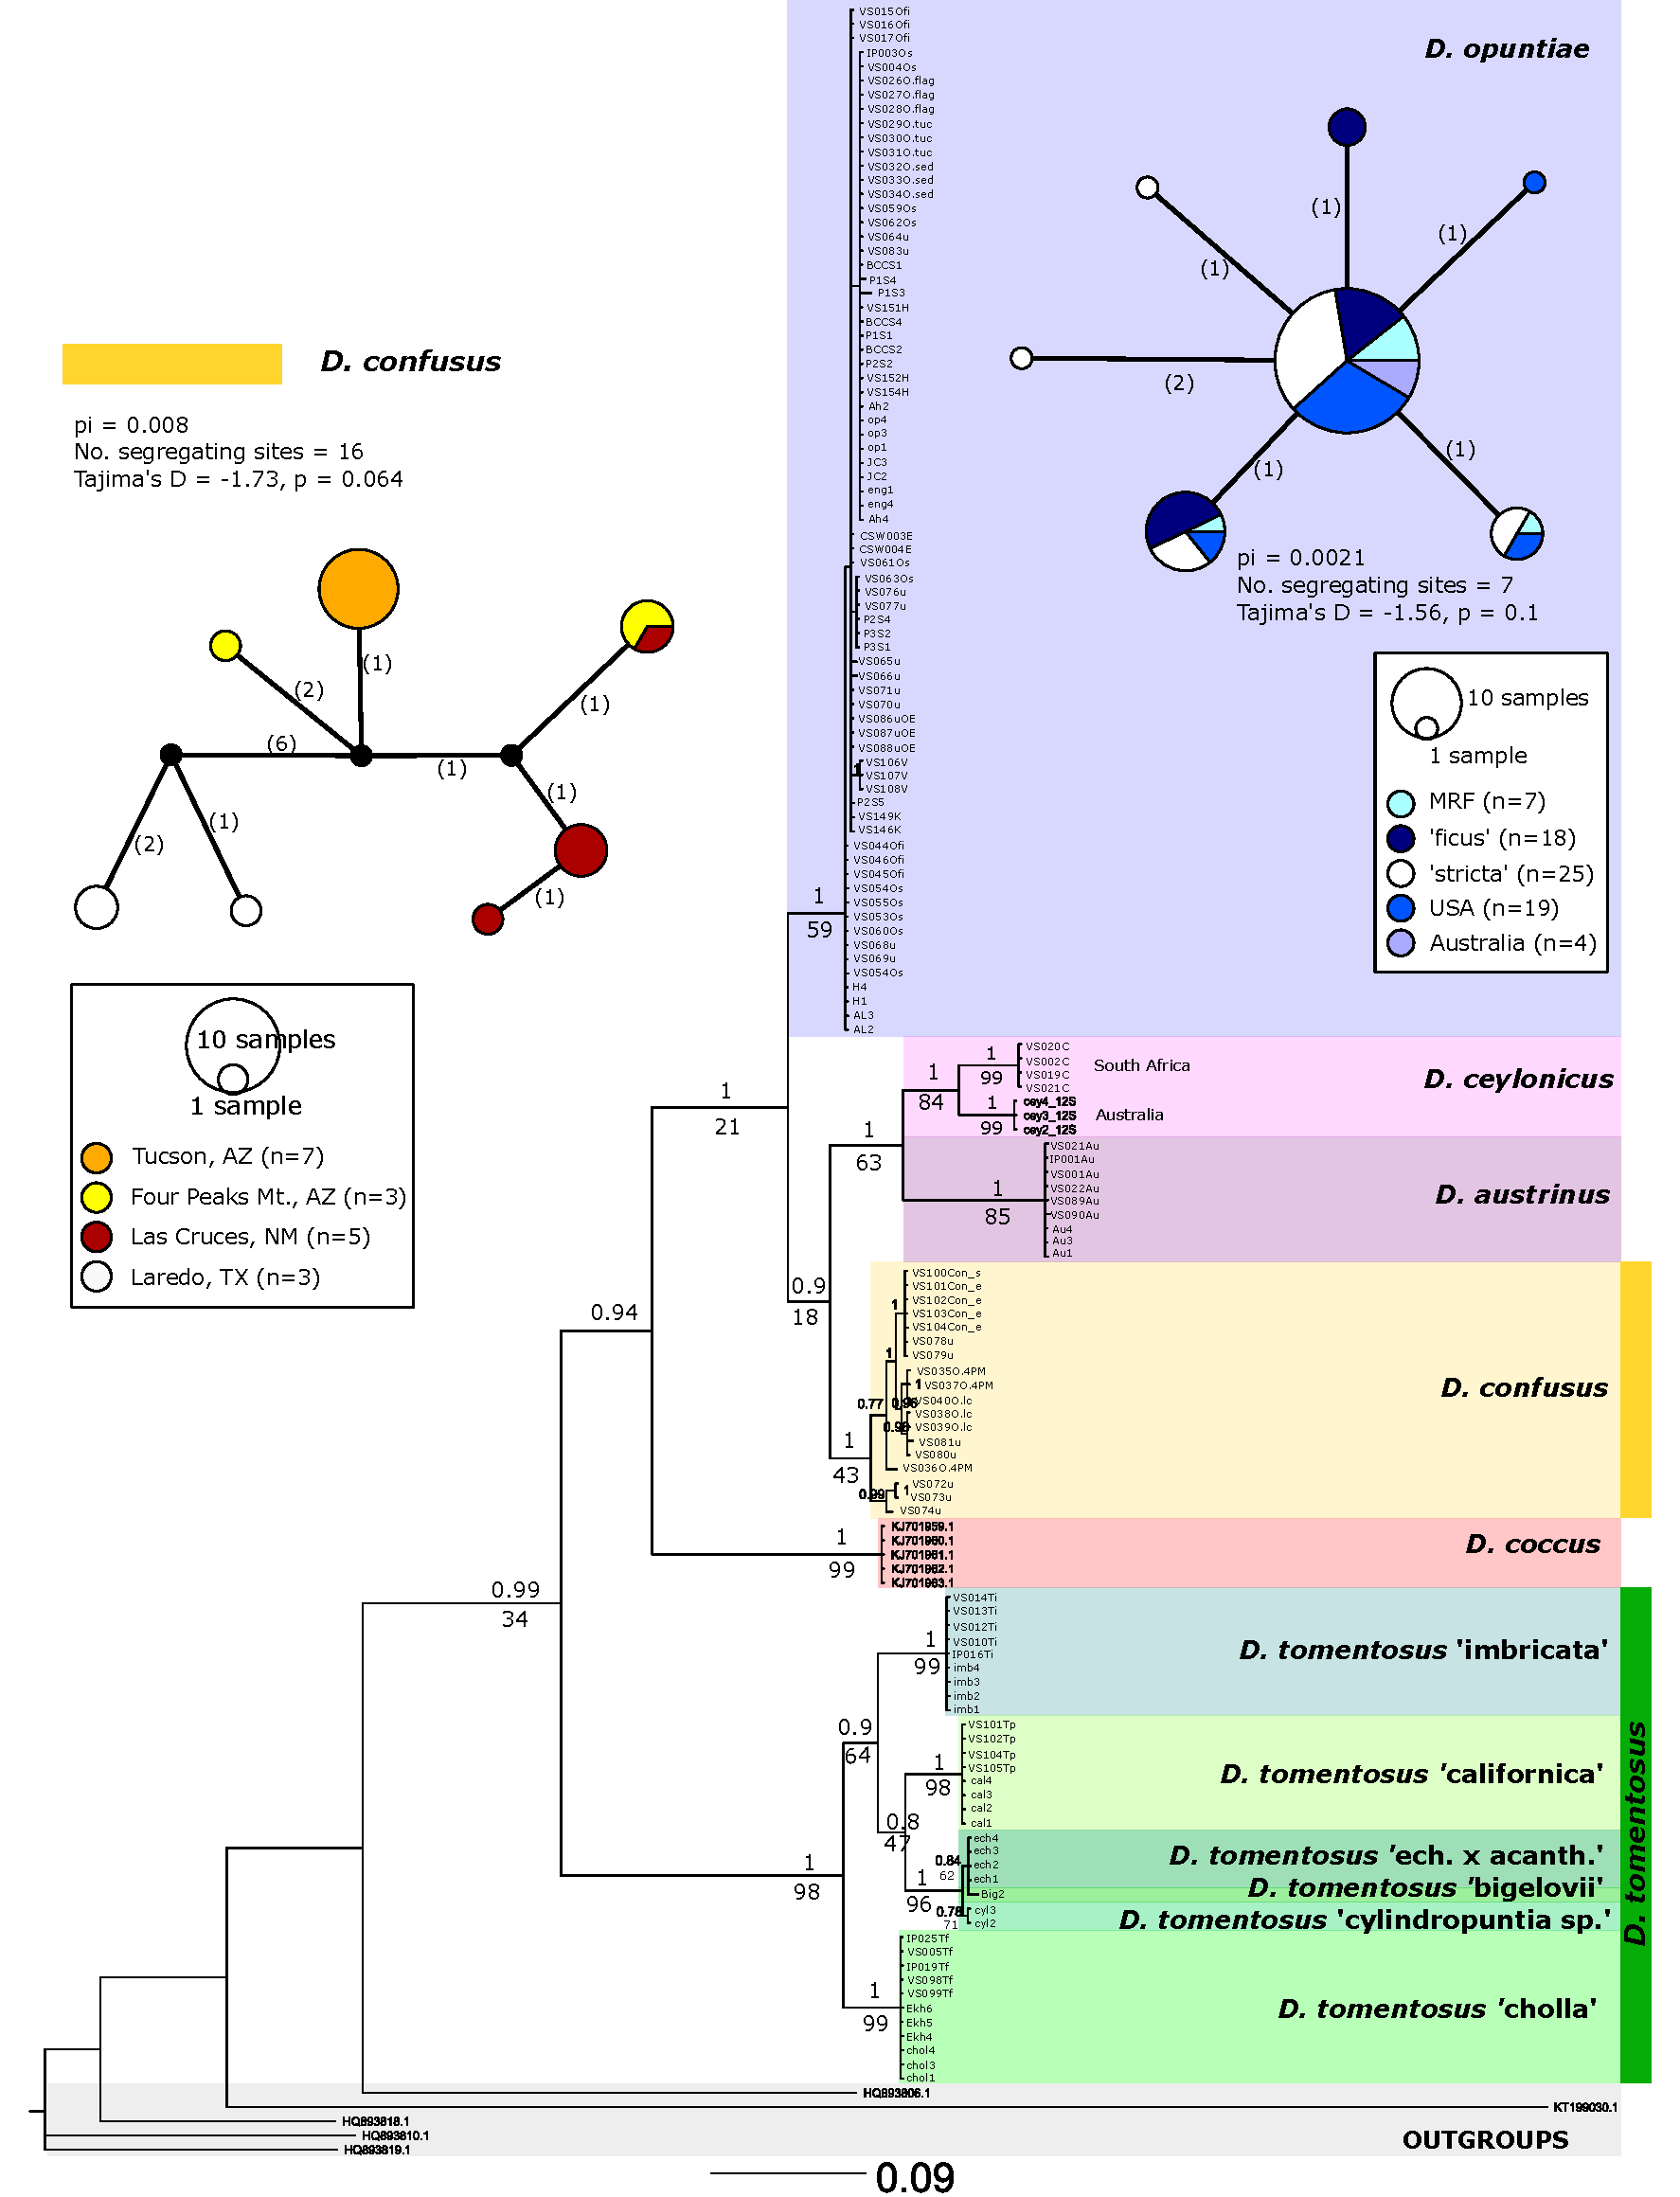
\includegraphics[scale =0.55]{Images/12S_MrBayes_2.pdf}
	\caption{Bayesian and Maximum likelihood phylogenies for the 12S gene region. Posterior probability values are above, and bootstrap values are below the branches. Haplotype networks are shown inset for \textit{D. opuntiae} and \textit{D. confusus}. Small black dots indicate missing haplotypes, and the diameter of each circle is proportional to the number of genetic sequences that comprise it. Numbers in brackets indicate the number of nucleotide differences between haplotypes.} 
	\label{fig:12S_tree}
\end{figure}

\clearpage
\begin{figure}[H]
	\centering
	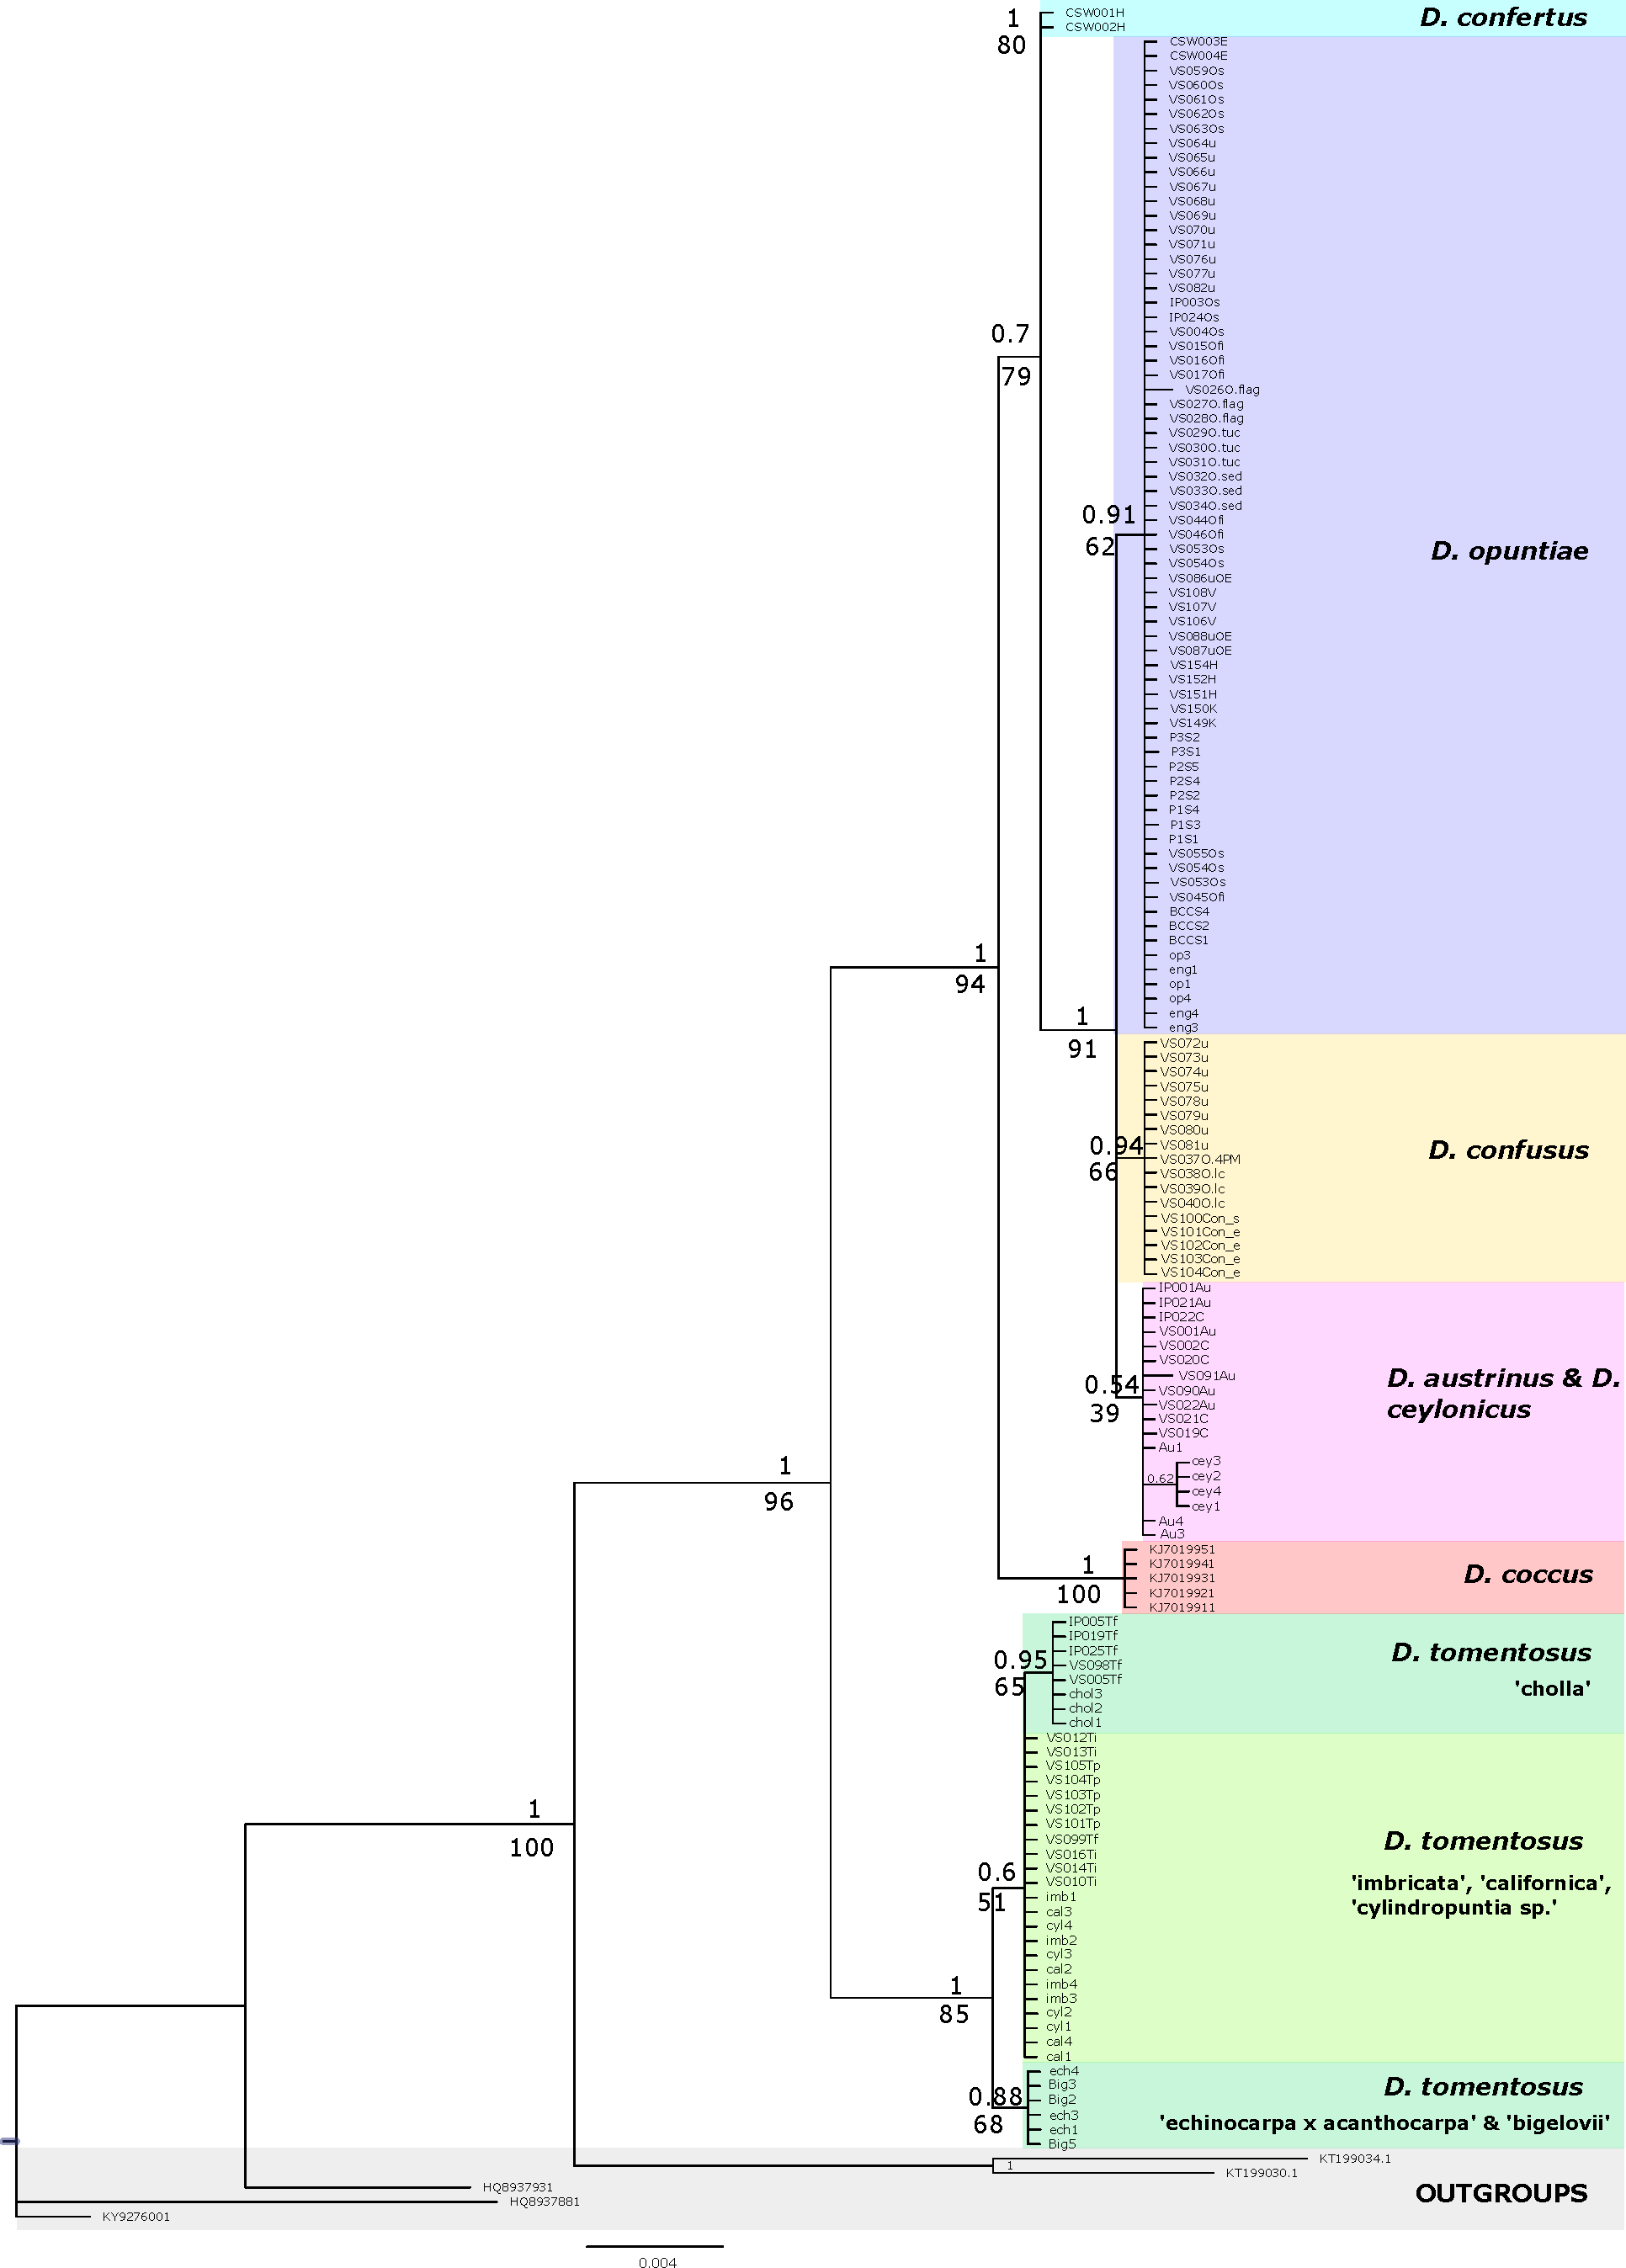
\includegraphics[scale =0.5]{Images/18S.pdf}
	\caption{Bayesian and Maximum likelihood  phylogenies for the 18S gene region. Posterior probability values are above, and bootstrap values are below the branches.} 
	\label{fig:18S_tree}
\end{figure}

\begin{figure}[H]
	\centering
	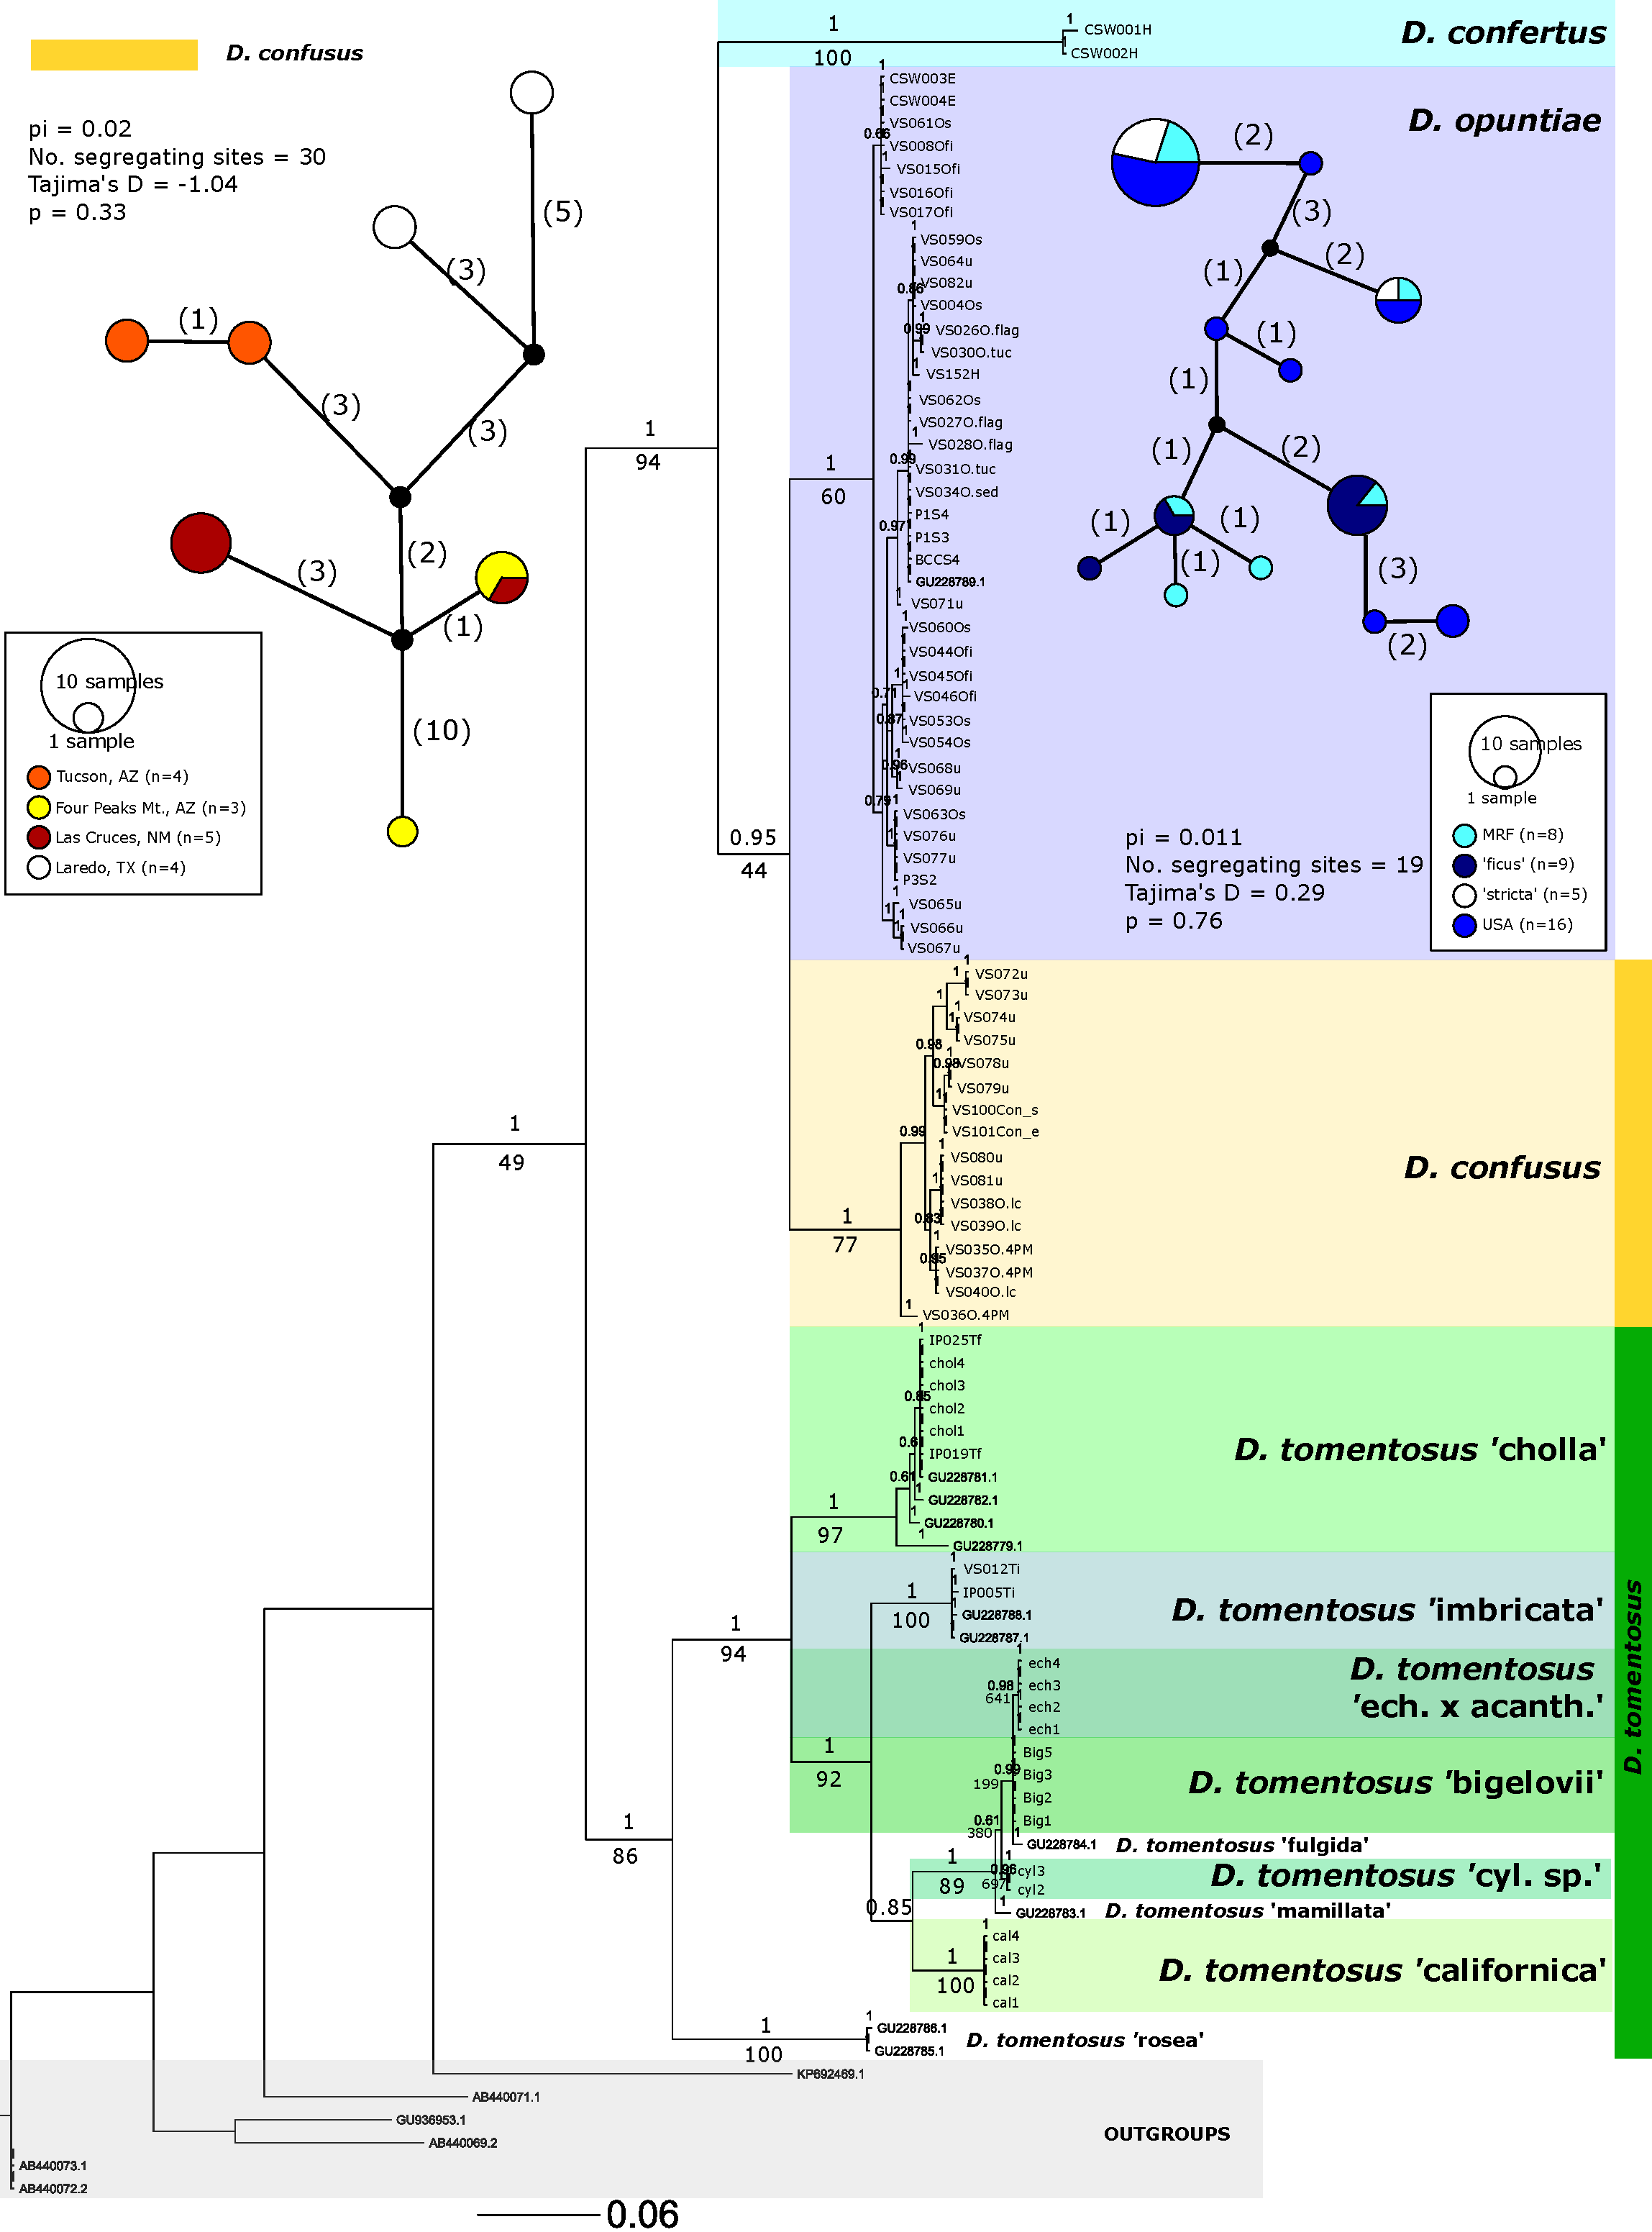
\includegraphics[scale =0.42]{Images/Bayesian_COI_both_primers.pdf}
	\caption{Bayesian and Maximum likelihood  phylogenies for the COI gene region. Posterior probabilities are above, and bootstrap values are below the branches. Haplotype networks are shown for \textit{D. opuntiae} and \textit{D. confusus}. Small black dots indicate missing haplotypes, and the diameter of each circle is proportional to the number of individuals it comprises. Numbers in brackets indicate the number of nucleotide differences between haplotypes.} 
	\label{fig:COI_tree}
\end{figure}

% \begin{landscape}

% \begin{figure}[H]
% 	\centering
% 	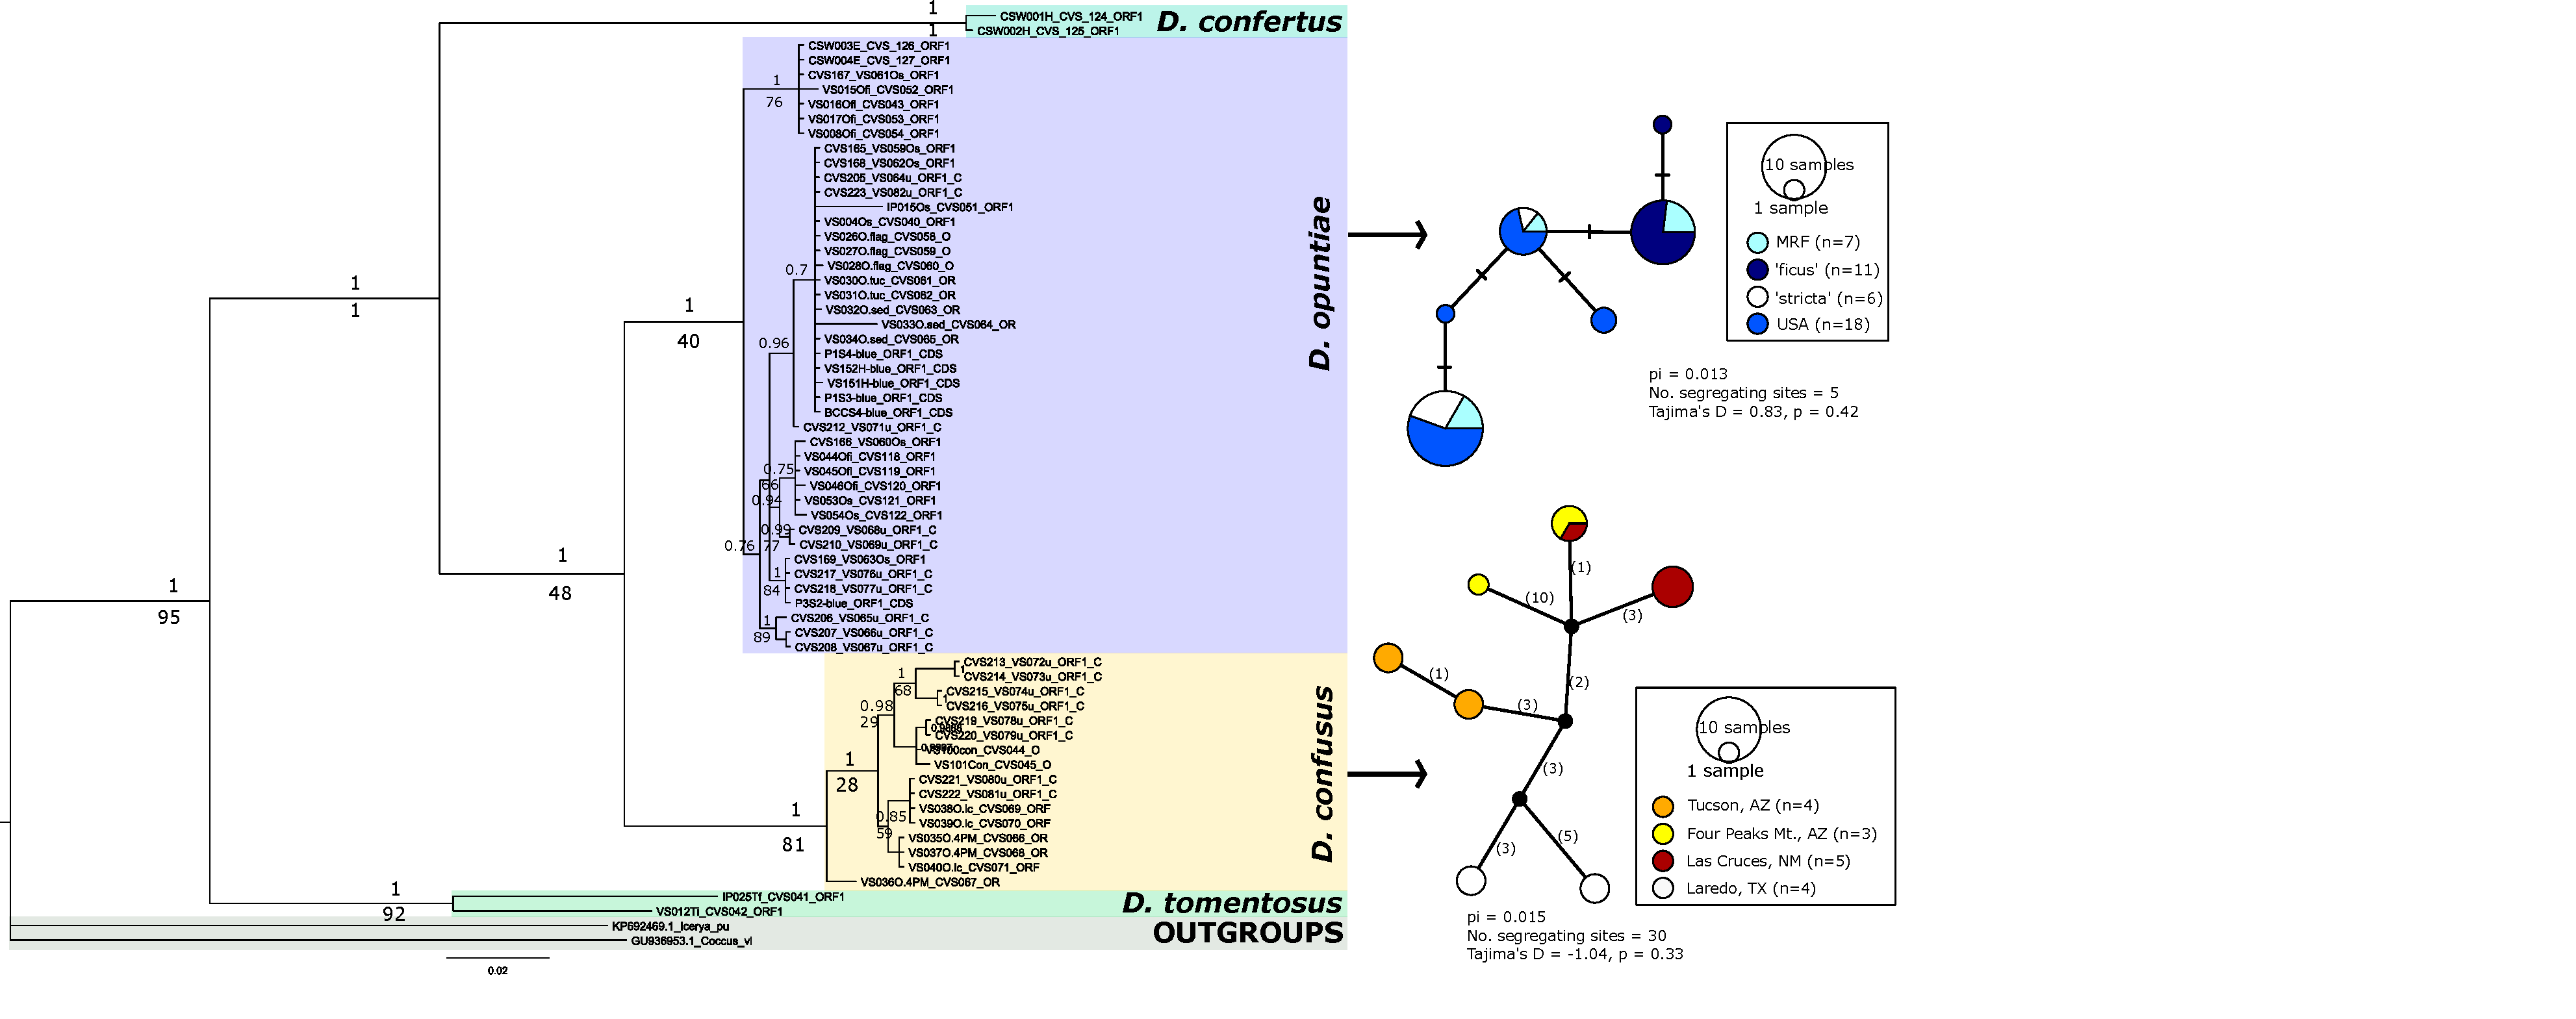
\includegraphics[scale =0.5]{Images/PCOF1.pdf}
% 	\caption{Bayesian (MrBayes) and Maximum likelihood (GARLI) phylogenetic trees for the COI (PCOF1 \& LepR1) gene. Bayesian posterior probability values are above, and Maximum likelihood bootstrap values are below the branches. Haplotype networks (using the TCS network method) are shown for \textit{D. opuntiae} and \textit{D. confusus}. Small black dots indicate missing haplotypes, and the diameter of each circle is proportional to the number of genetic sequences that share that particular haplotype. Hatch marks and numbers in brackets indicate the number of nucleotide differences between haplotypes.} 
% 	\label{fig:PCOF1_tree}
% \end{figure}

% \begin{figure}[H]
% \centering
% 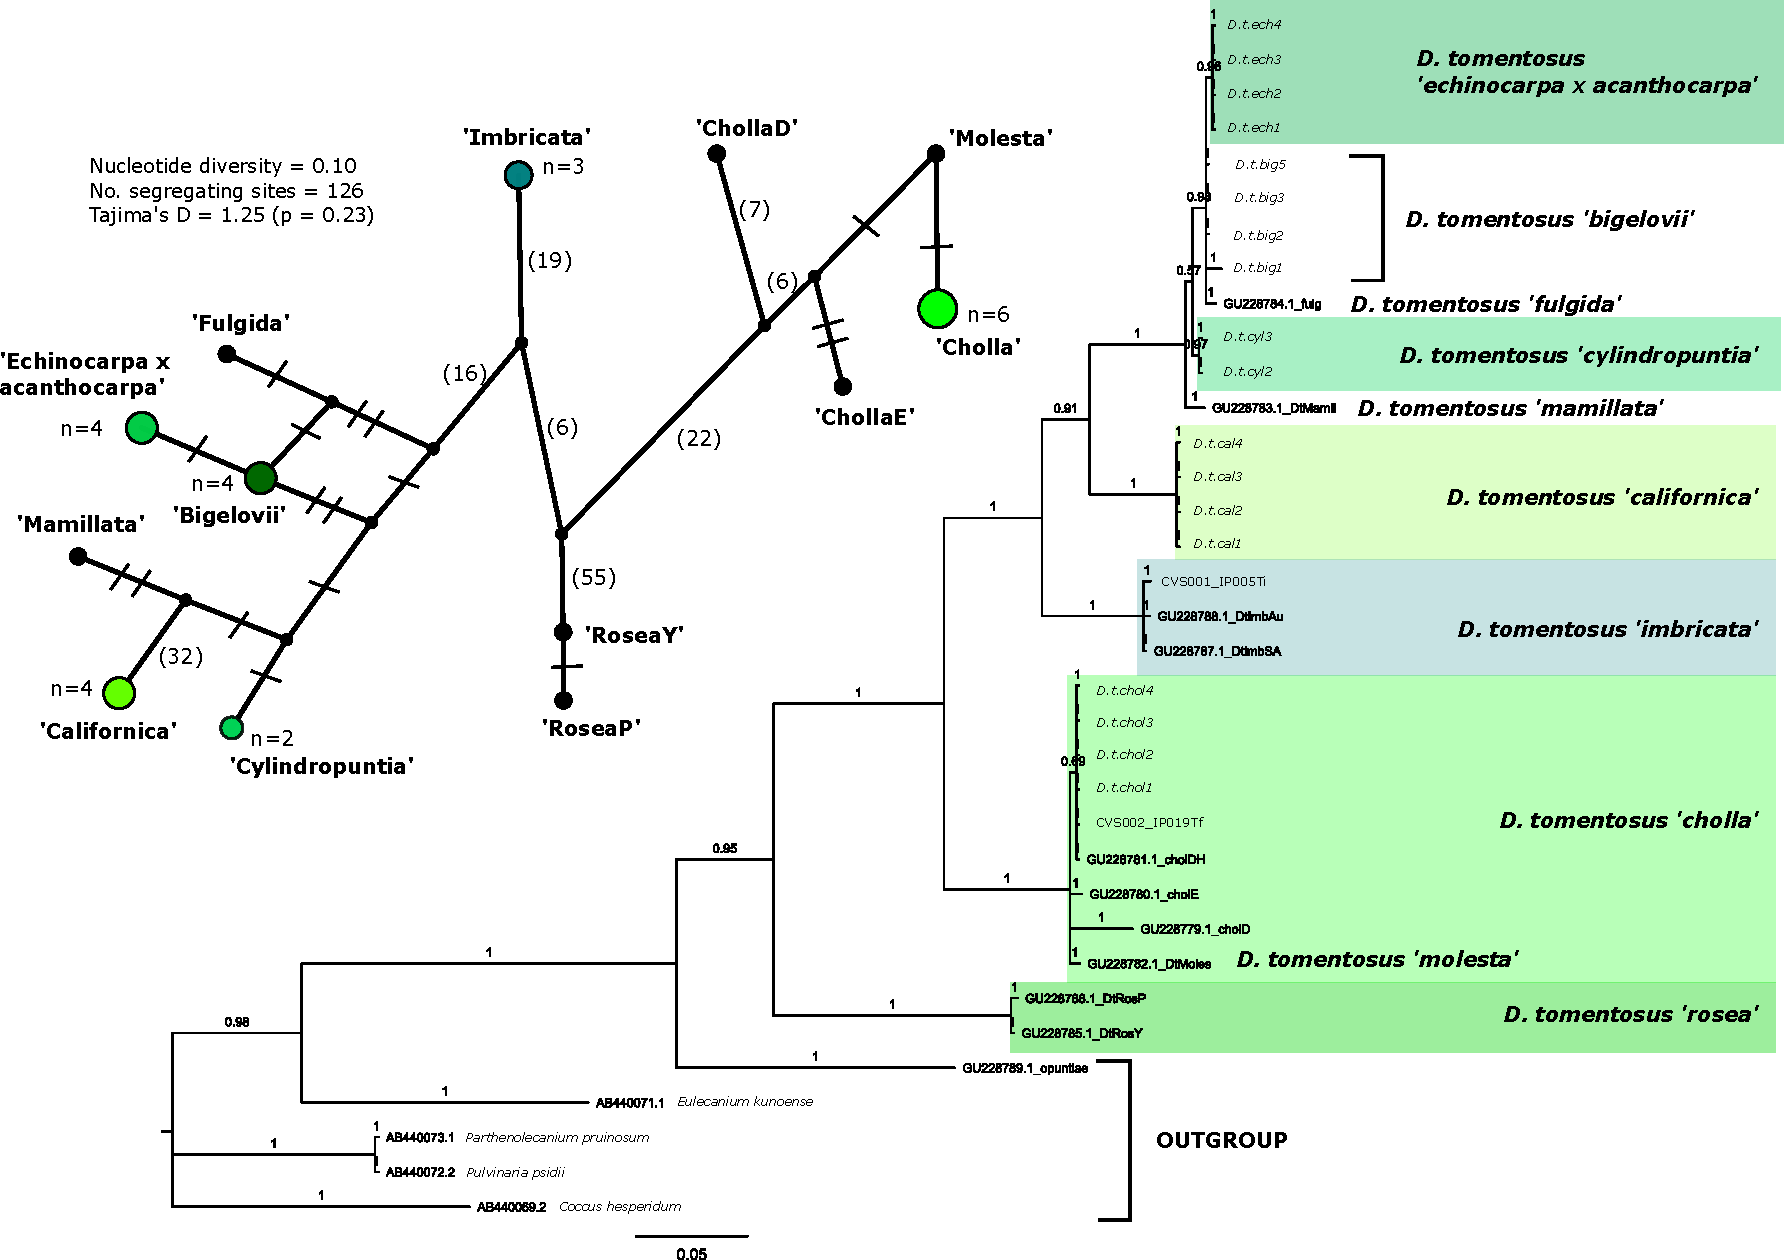
\includegraphics[scale = 0.75]{Images/COI_DTOM_BayesianTree.pdf}
% \caption{Bayesian phylogenetic tree for the COI(DTOMf \& HCO2198) gene. Posterior probabilities are shown on the branches. A haplotype network is shown alongside the tree (TCS network method) for \textit{D. tomentosus} lineages. Small black dots indicate missing haplotypes, and the diameter of each circle is proportional to the number of genetic sequences that share that particular haplotype. Hatch marks and numbers in brackets indicate the number of nucleotide differences between haplotypes.}
% \label{fig:COIDTOM_bayes}
% \end{figure}

% \begin{figure}[H]
% \centering
% 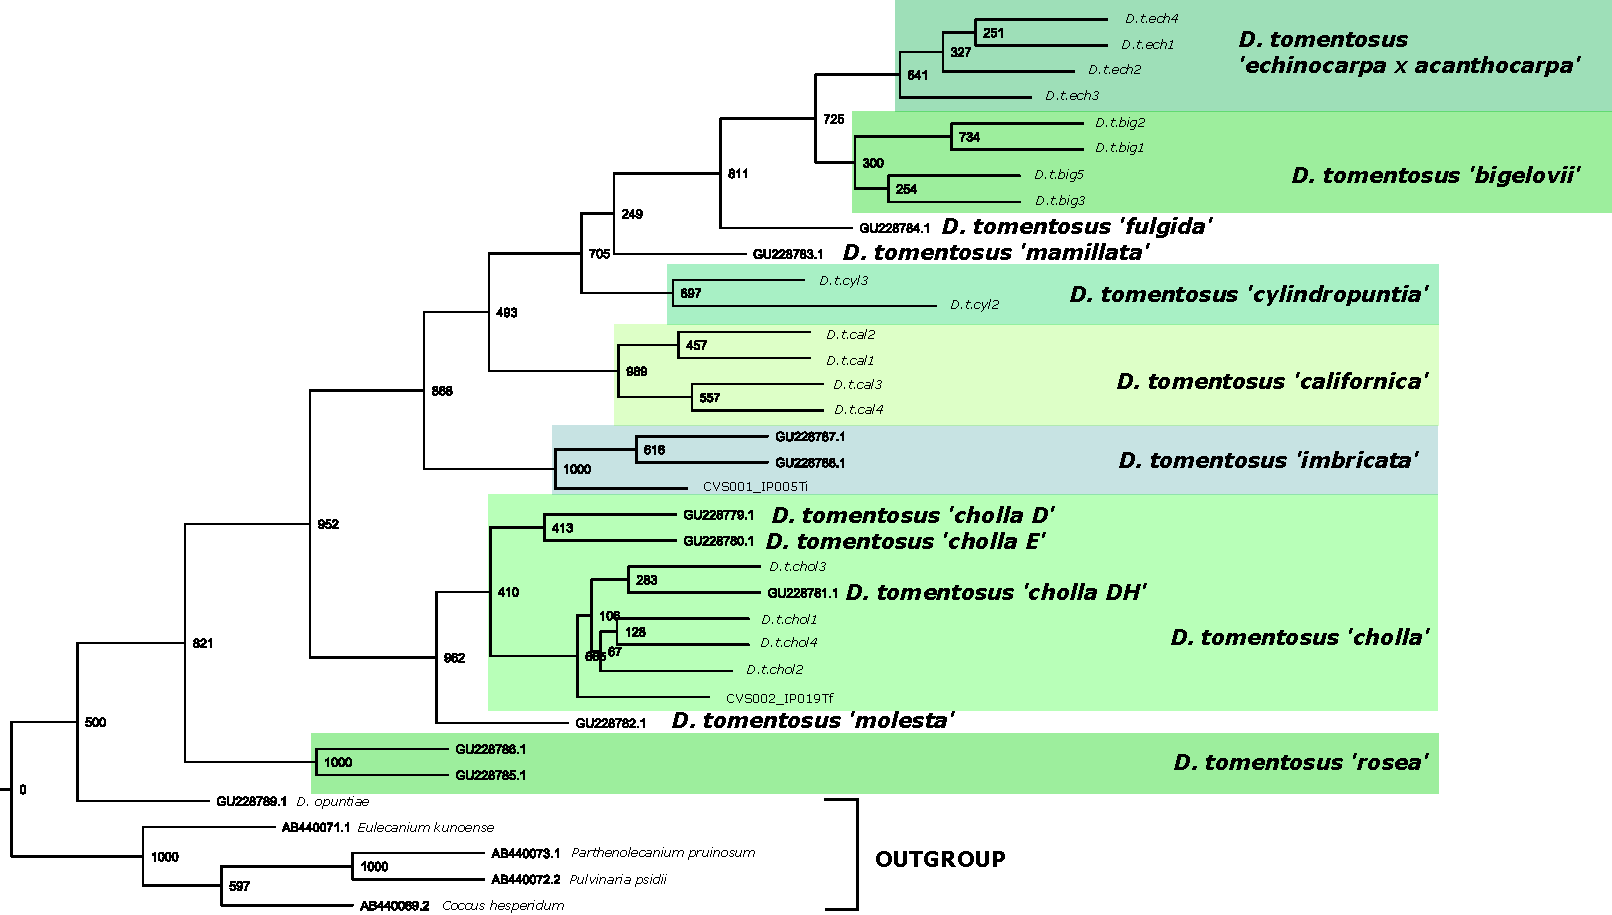
\includegraphics[scale = 0.85]{Images/COI_DTOM_GARLI.pdf}
% \caption{Maximum Likelihood phylogenetic tree for the COI(DTOMf \& HCO2198) gene. Bootstrap probabilities are shown on the branches.}
% \label{fig:COIDTOM_garli}
% \end{figure}

%  \end{landscape}

\begin{figure}[H]
	\centering
	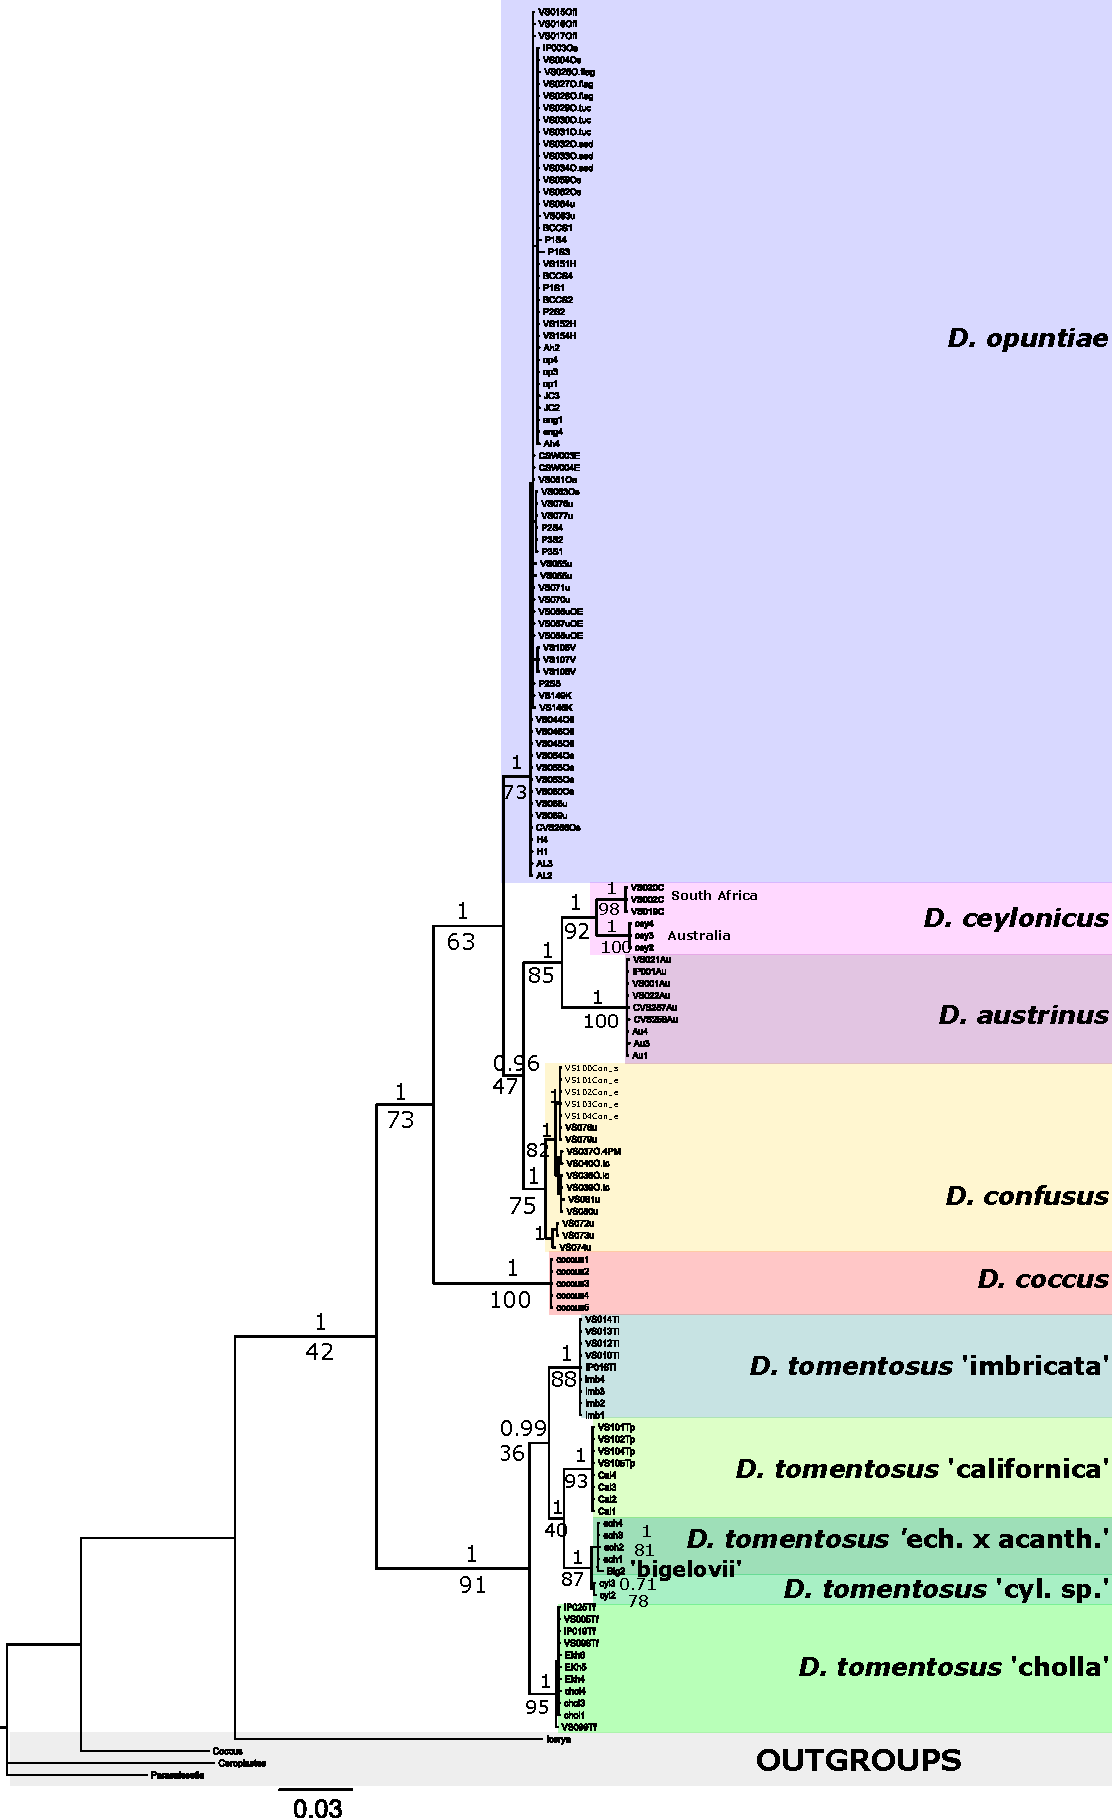
\includegraphics[scale =0.75]{Images/bayesian_concat2.pdf}
	\caption{Concatenated Bayesian and Maximum Likelihood phylogenies for the 12S and 18S gene regions. Bayesian posterior probability values are above, and Maximum likelihood bootstrap values are below the branches.} 
	\label{fig:concatTrees}
\end{figure}

\begin{landscape}
\begin{table}[H]
\renewcommand{\arraystretch}{0.4}
\caption{Within and between group p-distance matrix for the 12S gene, using the Kimura 2-parameter model. Species are represented by a total of 151 nucleotide sequences consisting of 779 positions. Bold values along the diagonal represent within-group p-distances.}
\label{tab:p_dist_12S}
\resizebox{\columnwidth}{!}{%
\begin{tabular}{@{}llllllllllll@{}}
\toprule
 & \textit{D. austrinus} & \textit{D. ceylonicus} & \textit{D. coccus} & \textit{D. confusus} & \textit{D. opuntiae} & \textit{D. tomentosus} `californica' & \textit{D. tomentosus} `cholla' & \textit{D. tomentosus} `cylindropuntia sp.' & \textit{D. tomentosus} `echinocarpa' & \textit{D. tomentosus} `imbricata' & Outgroup \\ \midrule
\begin{tabular}[l]{@{}l@{}} \textit{D. austrinus} \\ (n = 9) \end{tabular} & \textbf{0.000} &  &  &  &  &  &  &  &  &  &  \\
\begin{tabular}[l]{@{}l@{}} \textit{D. ceylonicus} \\ n = 6\end{tabular} & 0.17 & \textbf{0.050} &  &  &  &  &  &  &  &  &  \\
\begin{tabular}[l]{@{}l@{}} \textit{D. coccus} \\ n = 5\end{tabular} & 0.38 & 0.33 & \textbf{0.000} &  &  &  &  &  &  &  &  \\
\begin{tabular}[l]{@{}l@{}} \textit{D. confusus} \\ n = 18\end{tabular} & 0.17 & 0.16 & 0.30 & \textbf{0.015} &  &  &  &  &  &  &  \\
\begin{tabular}[l]{@{}l@{}} \textit{D. opuntiae} \\ n = 73\end{tabular} & 0.18 & 0.17 & 0.27 & 0.11 & \textbf{0.005} &  &  &  &  &  &  \\
\begin{tabular}[l]{@{}l@{}} \textit{D. tomentosus} `californica'\\ n = 8\end{tabular} & 0.42 & 0.39 & 0.41 & 0.39 & 0.42 & \textbf{0.000} &  &  &  &  &  \\
\begin{tabular}[l]{@{}l@{}} \textit{D. tomentosus} `cholla' \\ n = 12\end{tabular} & 0.39 & 0.38 & 0.39 & 0.37 & 0.39 & 0.13 & \textbf{0.068} &  &  &  &  \\
\begin{tabular}[l]{@{}l@{}} \textit{D. tomentosus} \\ `cylindropuntia sp.' \\ n = 2\end{tabular} & 0.42 & 0.41 & 0.41 & 0.40 & 0.40 & 0.09 & 0.14 & \textbf{0.000} &  &  &  \\
\begin{tabular}[l]{@{}l@{}} \textit{D. tomentosus} `echinocarpa' \\ n = 4\end{tabular} & 0.42 & 0.42 & 0.40 & 0.40 & 0.39 & 0.09 & 0.15 & 0.00 & \textbf{0.00} &  &  \\
\begin{tabular}[l]{@{}l@{}} \textit{D. tomentosus} `imbricata' \\ n = 9\end{tabular} & 0.44 & 0.40 & 0.40 & 0.41 & 0.42 & 0.10 & 0.13 & 0.09 & 0.09 & \textbf{0.00} &  \\
\begin{tabular}[l]{@{}l@{}} Outgroup \\ n = 5\end{tabular} & 0.70 & 0.66 & 0.71 & 0.65 & 0.67 & 0.73 & 0.75 & 0.73 & 0.71 & 0.74 & \textbf{0.903} \\ \bottomrule
\end{tabular}
}
\end{table}

\begin{table}[H]
\renewcommand{\arraystretch}{0.5}
\caption{Within and between group p-distance matrix for the 18S gene, using the Kimura 2-parameter model. Species are represented by a total of 153 nucleotide sequences consisting of 630 positions. Bold values along the diagonal represent within-group p-distances.}
\label{tab:p_dist_18S}
\resizebox{\columnwidth}{!}{%
\begin{tabular}{@{}lp{3.8cm}llllllll@{}}
\toprule
 & \begin{tabular}[c]{@{}l@{}} \textit{D. austrinus} \&\\ \textit{D. ceylonicus}  \end{tabular} & \textit{D. coccus} & \textit{D. confertus} & \textit{D. confusus} & \textit{D. opuntiae} & \textit{D. tomentosus} & \begin{tabular}[c]{@{}l@{}} \textit{D. tomentosus} `echinocarpa'\\ \& \textit{D. tomentosus} `bigelovii' \end{tabular} & \textit{D. tomentosus} `cholla' & Outgroup \\ \midrule
\begin{tabular}[c]{@{}l@{}} \textit{D. austrinus} \&\\ \textit{D. ceylonicus} (n=18) \end{tabular}  & \textbf{0.006} &  &  &  &  &  &  &  &  \\
\textit{D. coccus} (n=5)  & 0.033 & \textbf{0} &  &  &  &  &  &  &  \\
\textit{D. confertus} (n=2) & 0.016 & 0.020 & \textbf{0} &  &  &  &  &  &  \\
\textit{D. confusus} (n=17)  & 0.010 & 0.027 & 0.012 & \textbf{0} &  &  &  &  &  \\
\textit{D. opuntiae} (n=69)  & 0.010 & 0.028 & 0.013 & 0.004 & \textbf{0} &  &  &  &  \\
\textit{D. tomentosus} (n=31)  & 0.057 & 0.048 & 0.043 & 0.047 & 0.049 & \textbf{0} &  &  &  \\
\begin{tabular}[c]{@{}l@{}} \textit{D. tomentosus} `echinocarpa'\\ \& \textit{D. tomentosus} `bigelovii' (n=6) \end{tabular}  & 0.058 & 0.049 & 0.043 & 0.047 & 0.050 & 0.004 & \textbf{0} &  &  \\
\textit{D. tomentosus} `cholla' (n=5)  & 0.059 & 0.047 & 0.045 & 0.049 & 0.051 & 0.002 & 0.005 & \textbf{0} &  \\
Outgroup (n=5) & 0.134 & 0.129 & 0.123 & 0.125 & 0.127 & 0.114 & 0.117 & 0.116 & \textbf{0.114} \\ \bottomrule
\end{tabular}
}
\end{table}
\end{landscape}

\begin{landscape}

\begin{table}[]
\renewcommand{\arraystretch}{0.5}
\caption{Within and between group p-distance matrix for the COI-A and COI-B regions, using the Kimura 2-parameter model. Species are represented by a total of 95 nucleotide sequences consisting of 603 positions. Bold values along the diagonal represent within-group p-distances.}
\label{tab:p_dist_COI}
\centering
 \resizebox{\columnwidth}{!}{%
\begin{tabular}{@{}llllllllllll@{}}
\toprule
 & \textit{D. confusus} & \textit{D. confertus} & \textit{D. opuntiae} & \begin{tabular}[c]{@{}l@{}} \textit{D. tomentosus} \\ `bigelovii'\end{tabular} & \begin{tabular}[c]{@{}l@{}} \textit{D. tomentosus} \\ `californica'\end{tabular} & \begin{tabular}[c]{@{}l@{}} \textit{D. tomentosus} \\ `cholla'\end{tabular} & \begin{tabular}[c]{@{}l@{}} \textit{D. tomentosus} \\ `cylindropuntia sp.'\end{tabular} & \begin{tabular}[c]{@{}l@{}} \textit{D. tomentosus} \\ `echinocarpa'\end{tabular} & \begin{tabular}[c]{@{}l@{}} \textit{D. tomentosus} \\ `imbricata'\end{tabular} & \begin{tabular}[c]{@{}l@{}} \textit{D. tomentosus} \\ 'rosea'\end{tabular} & Outgroups \\ \midrule
\textit{D. confusus} (n=16) & \textbf{0.017} &  &  &  &  &  &  &  &  &  &  \\
\textit{D. confertus} (n=2) & 0.29 & \textbf{0.008} &  &  &  &  &  &  &  &  &  \\
\textit{D. opuntiae} (n=39) & 0.13 & 0.28 & \textbf{0.014} &  &  &  &  &  &  &  &  \\
\textit{D. tomentosus} `bigelovii' (n=4) & 0.24 & 0.36 & 0.23 & \textbf{0.000} &  &  &  &  &  &  &  \\
\textit{D. tomentosus} `californica' (n=4) & 0.24 & 0.31 & 0.24 & 0.09 & \textbf{0.000} &  &  &  &  &  &  \\
\textit{D. tomentosus} `cholla' (n=9) & 0.27 & 0.36 & 0.25 & 0.14 & 0.14 & \textbf{0.009} &  &  &  &  &  \\
\textit{D. tomentosus} `cylindropuntia sp.' (n=2) & 0.24 & 0.36 & 0.24 & 0.01 & 0.09 & 0.15 & \textbf{0.000} &  &  &  &  \\
\textit{D. tomentosus} `echinocarpa' (n=4) & 0.25 & 0.37 & 0.23 & 0.00 & 0.10 & 0.15 & 0.01 & \textbf{0.000} &  &  &  \\
\textit{D. tomentosus} `imbricata' (n=4) & 0.26 & 0.34 & 0.23 & 0.10 & 0.11 & 0.14 & 0.10 & 0.10 & \textbf{0.002} &  &  \\
\textit{D. tomentosus} `rosea' (n=2) & 0.25 & 0.31 & 0.25 & 0.22 & 0.23 & 0.21 & 0.23 & 0.22 & 0.21 & \textbf{0.002} &  \\
Outgroups & 0.34 & 0.44 & 0.32 & 0.34 & 0.33 & 0.32 & 0.34 & 0.34 & 0.32 & 0.31 & \textbf{0.235} \\ \bottomrule
\end{tabular}
}
\end{table}


% \begin{table}[H]
% \renewcommand{\arraystretch}{0.5}
% \caption{Within and between group p-distance matrix for the COI (DTOMf \& HCO2198) gene, using the Kimura 2-paramter model. Species are represented by a total of 32 nucleotide sequences consisting of 546 positions. Bold values along the diagonal represent within group p-distances.}
% \label{tab:p_dist_dtom}
% \resizebox{\columnwidth}{!}{%
% \begin{tabular}{@{}lllllllll@{}}
% \toprule
%  & \textit{\begin{tabular}[c]{@{}l@{}}D. tomentosus 'echinocarpa x \\ acanthocarpa'\end{tabular}} & \textit{\begin{tabular}[c]{@{}l@{}}D. tomentosus \\ 'cylindropuntia'\end{tabular}} & \textit{\begin{tabular}[c]{@{}l@{}}D. tomentosus \\ 'cholla'\end{tabular}} & \textit{\begin{tabular}[c]{@{}l@{}}D. tomentosus \\ 'californica'\end{tabular}} & \textit{\begin{tabular}[c]{@{}l@{}}D. tomentosus \\ 'bigelovii'\end{tabular}} & \textit{\begin{tabular}[c]{@{}l@{}}D. tomentosus \\ 'imbricata'\end{tabular}} & \textit{\begin{tabular}[c]{@{}l@{}}D. tomentosus \\ 'rosea'\end{tabular}} & Outgroup \\ \midrule
% \textit{\begin{tabular}[c]{@{}l@{}}D. tomentosus 'echinocarpa x \\ acanthocarpa' (n=4)\end{tabular}} & \textbf{0} &  &  &  &  &  &  &  \\
% \textit{\begin{tabular}[c]{@{}l@{}}D. tomentosus \\ 'cylindropuntia' (n=2)\end{tabular}} & 0.011 & \textbf{0} &  &  &  &  &  &  \\
% \textit{\begin{tabular}[c]{@{}l@{}}D. tomentosus \\ 'cholla' (n=8)\end{tabular}} & 0.146 & 0.152 & \textbf{0.1} &  &  &  &  &  \\
% \textit{\begin{tabular}[c]{@{}l@{}}D. tomentosus \\ 'californica' (n=4)\end{tabular}} & 0.096 & 0.089 & 0.139 & \textbf{0} &  &  &  &  \\
% \textit{\begin{tabular}[c]{@{}l@{}}D. tomentosus \\ 'bigelovii' (n=4)\end{tabular}} & 0.004 & 0.010 & 0.145 & 0.094 & \textbf{0.003} &  &  &  \\
% \textit{\begin{tabular}[c]{@{}l@{}}D. tomentosus \\ 'imbricata' (n=3)\end{tabular}} & 0.102 & 0.102 & 0.143 & 0.105 & 0.100 & \textbf{0.003} &  &  \\
% \textit{\begin{tabular}[c]{@{}l@{}}D. tomentosus \\ 'rosea' (n=2)\end{tabular}} & 0.218 & 0.226 & 0.213 & 0.222 & 0.216 & 0.212 & \textbf{0.002} &  \\
% \begin{tabular}[c]{@{}l@{}}Outgroup \\ (n=5)\end{tabular} & 0.317 & 0.313 & 0.298 & 0.312 & 0.314 & 0.296 & 0.288 & \textbf{0.23} \\ \bottomrule
% \end{tabular}
% }
% \end{table}

\end{landscape}

\section{Identification accuracy}

\subsection{Nearest Neighbour (NN) results}
For species-level identification at a default distance threshold of 1\%, the NN algorithm can be a useful test of accuracy. However, when different genes are being analysed that display different evolutionary rates, an adjustable threshold value is required. The NN algorithm tends to result in an abnormally high number of false positive identifications, and is therefore not considered further. For example, Table \ref{tab:barcode_test_results} shows a NN `True' outcome of 88.46\% for the correct identification of the \textit{D. opuntiae} lineages using the COI region, while the more stringent TID test only had an accuracy rate of 59.62\% at a lower threshold of 0.8\%.  

\subsection{12S}
At the species level, and at the optimal genetic distance threshold of 1\%, identification accuracy (IA) was 100\% for both barcode tests (BCM and TID) (Table \ref{tab:barcode_test_results}). At the lineage level, \textit{Dactylopius tomentosus} had an IA of 100\% (BCM) and 82.4\% (TID) at a distance threshold of 1\%. The TID result increased to 100\% at a lower optimal threshold value of 0.2\%. \textit{Dactylopius opuntiae} only had an IA of 15.22\% (with ambiguities at 82.61\% and incorrect IDs at 2.17\%) for the BCM test and a zero IA (100\% ambiguities) for the TID test at a threshold of 1\%. At a decreased threshold of 0.2\%, the TID only increased to a 13.04\% IA, with amibiguities at 80.43\% (incorrect and no IDs at 2.17\% and 4.35\%, respectively). The range of threshold genetic distance values for the \textit{D. opuntiae} lineages all showed a high occurrence of false negatives. 
Barcode gaps at the species level and for \textit{D. tomentosus} lineages were all positive (i.e., interspecific $>$ intraspecific variation), while the lineages within \textit{D. opuntiae} were all negative (i.e., interspecific $<$ intraspecific variation). Of the \textit{D. tomentosus} lineages, the `cylindropuntia sp.' and `echinocarpa x acanthocarpa' lineages had the smallest barcode gaps. 

\subsection{18S}
At the species level, and at the default genetic threshold of 1\%, IA was 94.59\% (5.41\% ambiguity) for the BCM test, but only 29.73\% (70.27\% ambiguities) for the TID test (Table \ref{tab:barcode_test_results}). At a lower threshold of 0.2\%, the IA for both the BCM and TID tests were 94.59\%, with ambiguities of 5.41\%. At the lineage level, at a threshold of 0.1\%, \textit{D. tomentosus} had an IA of 22.22\% (77.78\% ambiguities) for both the BCM and TID tests. The intraspecific lineages of \textit{Dactylopius opuntiae} produced 100\% ambiguous results for the BCM and TID tests at the 0.1\% threshold. The range of genetic threshold distance values for the lineages within \textit{D. tomentosus} and \textit{D. opuntiae} all showed a high number of false negatives. 
Barcode gaps at the species level were all positive, except for \textit{D. austrinus} and \textit{D. ceylonicus} sequences, which had negative barcode gaps (as illustrated in the phylogenetic tree in Figure \ref{fig:18S_tree}). The largest positive barcode gaps at the species level were for \textit{D. tomentosus}. Barcode gaps for \textit{D. opuntiae} and \textit{D. tomentosus} at the lineage level were all zero (i.e., the intra-and interspecific variation in these groups were equal); except for \textit{D. tomentosus} `cholla' sequences, which had positive barcode gaps. 

\subsection{COI}
Identification accuracy at the species level at a 1\% threshold was 100\% for both the BCM and TID tests (Table \ref{tab:barcode_test_results}). At the lineage level, at a 1\% threshold, \textit{D. opuntiae} had an IA of 61.54\% (32.69\% ambiguities and 5.77\% incorrect) for the BCM test, and an IA of 46.15\% (51.92\% ambiguities and 1.92\% incorrect) for the TID test. The BCM test results remained the same at a lower optimal threshold of 0.8\%, but the TID IA rose to 59.62\% (38.46\% ambiguities and 1.92\% incorrect). 
At the lineage level for \textit{D. tomentosus}, when `bigelovii', `cylindropuntia sp.', and `echinocarpa x acanthocarpa' were treated as separate lineages, IA was 96.3\% (3.7\% ambiguities) for the BCM test, and 59.26\% (37.04\% ambiguities and 3.7\% no ID) for the TID test (Table \ref{tab:barcode_test_results}). At a lower threshold value of 0.2\%, the BCM decreased to an IA of 88.89\% (11.11\% ambiguities), and the TID rose to 70.37\% (18.52\% ambiguities and 11.11\% no ID). When `bigelovii', `cylindropuntia sp.', and `echinocarpa x acanthocarpa' were treated as one group, at a threshold of 3.3\%, the IA for both the BCM and TID tests was 100\%. 
Barcode gaps were positive for all sequences at the species level, but negative for all \textit{D. opuntiae} sequences at the lineage level. Barcode gaps for \textit{D. tomentosus} lineages were all positive except for three `bigelovii' sequences.

\begin{landscape}

\begin{table}[!htp]
\renewcommand{\arraystretch}{0.5}
\caption{Results of the Best Close Match (BCM), Threshold ID (TID) and Nearest Neighbour (NN) barcode testing algorithms for the 12S, 18S and COI gene regions. Values for BCM and TID are shown at the default 1\% and at the optimum threshold value. Results are shown at the species and lineage level. In the COI section, \textit{D. tomentosus} (G) indicates a test conducted where the `bigelovii', `cylindropuntia sp.', and `echinocarpa x acanthocarpa' sequences were grouped as one lineage.}
\label{tab:barcode_test_results}
\resizebox{\columnwidth}{!}{%
\begin{tabular}{@{}llllllllllllll@{}}
\toprule
 &  & \textbf{BCM} & \textbf{\begin{tabular}[c]{@{}l@{}}Proportion of\\   samples (\%)\end{tabular}} & \textbf{TID (1\%)} & \textbf{\begin{tabular}[c]{@{}l@{}}Proportion of\\   samples (\%)\end{tabular}} & \textbf{BCM (optimum \%)} & \textbf{\begin{tabular}[c]{@{}l@{}}Proportion of\\   samples (\%)\end{tabular}} & \textbf{TID (optimum \%)} & \textbf{\begin{tabular}[c]{@{}l@{}}Proportion of\\   samples (\%)\end{tabular}} & \textbf{} & \textbf{} & \textbf{NN} & \textbf{\begin{tabular}[c]{@{}l@{}}Proportion of\\   samples (\%)\end{tabular}} \\ \midrule
\multicolumn{14}{c}{\textbf{12S}} \\ \midrule
\textbf{\begin{tabular}[c]{@{}l@{}}SPECIES\\   LEVEL\end{tabular}} & \textbf{Correct} & 147 & 100 & 147 & 100 &  &  &  &  &  & \textbf{T} & 147 & 100 \\
 &  &  &  &  &  &  &  &  &  &  & \textbf{F} & 0 & 0 \\
% \textbf{LINEAGE LEVEL (overall)} &  &  &  &  &  & \textbf{0.2\%} &  & \textbf{0.2\%} &  &  &  &  &  \\
%  & \textbf{Correct} & 78 & 53.06 & 67 & 45.58 & 73 & 49.66 & 73 & 49.66 &  &  &  &  \\
%  & \textbf{Incorrect} & 2 & 1.36 & 0 & 0 & 1 & 0.68 & 1 & 0.68 &  & \textbf{T} & 110 & 74.83 \\
%  & \textbf{Ambiguous} & 67 & 45.58 & 80 & 54.42 & 65 & 44.22 & 65 & 44.22 &  & \textbf{F} & 37 & 25.17 \\
%  & \textbf{No id} & 0 & 0 & 0 & 0 & 8 & 5.44 & 8 & 5.44 &  &  &  &  \\
\textbf{LINEAGE LEVEL} &  &  &  &  &  &  &  &  &  &  &  &  &  \\
 & \textit{\textbf{D. opuntiae}} &  &  &  &  & \textbf{0.2\%} &  & \textbf{0.2\%} &  &  &  &  &  \\
 & \textbf{Correct} & 7 & 15.22 & 0 & 0 & 6 & 13.04 & 6 & 13.04 &  & \textbf{T} & 37 & 80.43 \\
 & \textbf{Incorrect} & 1 & 2.17 & 0 & 0 & 1 & 2.17 & 1 & 2.17 &  & \textbf{F} & 9 & 19.57 \\
 & \textbf{Ambiguous} & 38 & 82.61 & 46 & 100 & 37 & 80.43 & 37 & 80.43 &  &  &  &  \\
 & \textbf{No id} & 0 & 0 & 0 & 0 & 2 & 4.35 & 2 & 4.35 &  &  &  &  \\
 & \textit{\textbf{D. tomentosus}} &  &  &  &  &  &  & \textbf{0.2\%} &  &  &  &  &  \\
 & \textbf{Correct} & 34 & 100.0 & 28 & 82.4 &  &  & 34 & 100.0 &  & \textbf{T} & 34 & 100.0 \\
 & \textbf{Incorrect} & 0 & 0.0 & 0 & 0.0 &  &  & 0 & 0.0 &  & \textbf{F} & 0 & 0 \\
 & \textbf{Ambiguous} & 0 & 0.0 & 6 & 17.6 &  &  & 0 & 0.0 &  &  &  &  \\
 &  &  &  &  &  &  &  &  &  &  &  &  &  \\ \midrule
\multicolumn{14}{c}{\textbf{18S}} \\ \midrule
 &  &  &  &  &  & \textbf{0.2\%} &  & \textbf{0.2\%} &  &  &  &  &  \\
\textbf{\begin{tabular}[c]{@{}l@{}}SPECIES\\   LEVEL\end{tabular}} & \textbf{Correct} & 140 & 94.59 & 44 & 29.73 & 140 & 94.59 & 140 & 94.59 &  & \textbf{T} & 148 & 100 \\
 & \textbf{Ambiguous} & 8 & 5.41 & 104 & 70.27 & 8 & 5.41 & 8 & 5.41 &  & \textbf{F} & 0 & 0 \\
 &  &  &  &  &  &  &  &  &  &  &  &  &  \\
% \textbf{LINEAGE LEVEL (overall)} &  &  &  &  &  & \textbf{0.1\%} &  & \textbf{0.1\%} &  &  &  &  &  \\
%  & \textbf{Correct} & 42 & 28.38 & 7 & 4.73 & 41 & 27.70 & 41 & 27.70 &  &  &  &  \\
%  & \textbf{Incorrect} & 1 & 0.68 & 0 & 0 & 1 & 0.68 & 1 & 0.68 &  & \textbf{T} & 77 & 52.03 \\
%  & \textbf{Ambiguous} & 105 & 70.95 & 141 & 95.27 & 105 & 70.95 & 105 & 70.95 &  & \textbf{F} & 71 & 47.97 \\
%  & \textbf{No id} & 0 & 0 & 0 & 0 & 1 & 0.68 & 1 & 0.68 &  &  &  &  \\
\textbf{LINEAGE LEVEL} &  &  &  &  &  &  &  &  &  &  &  &  &  \\
 & \textit{\textbf{D. opuntiae}} &  &  &  &  &  &  & \textbf{0.1\%} &  &  &  &  &  \\
 & \textbf{Correct} &  &  & 0 & 0 &  &  & 0 & 0 &  &  &  &  \\
 & \textbf{Incorrect} &  &  & 0 & 0 &  &  & 0 & 0 &  &  &  &  \\
 & \textbf{Ambiguous} &  &  & 35 & 100 &  &  & 35 & 100 &  &  &  &  \\
 & \textbf{No id} &  &  & 0 & 0 &  &  & 0 & 0 &  &  &  &  \\
 & \textit{\textbf{D. tomentosus}} &  &  &  &  & \textbf{0.1\%} &  & \textbf{0.1\%} &  &  &  &  &  \\
 & \textbf{Correct} & 8 & 22.22 & 0 & 0 & 8 & 22.22 & 8 & 22.22 &  & \textbf{T} & 8 & 22.22 \\
 & \textbf{Incorrect} & 0 & 0 & 0 & 0 & 0 & 0 & 0 & 0 &  & \textbf{F} & 28 & 77.78 \\
 & \textbf{Ambiguous} & 28 & 77.78 & 36 & 100 & 28 & 77.78 & 28 & 77.78 &  &  &  &  \\
 &  &  &  &  &  &  &  &  &  &  &  &  &  \\ \midrule
\multicolumn{14}{c}{\textbf{COI}} \\ \midrule
\textbf{SPECIES LEVEL} & \textbf{Correct} & 83 & 100 & 83 & 100 &  &  &  &  &  & \textbf{T} & 83 & 100 \\
 &  &  &  &  &  &  &  &  &  &  & \textbf{F} & 0 & 0 \\
\textbf{LINEAGE LEVEL} & \textit{\textbf{D. opuntiae}}  &  &  &  &  & \textbf{0.8\%} &  & \textbf{0.8\%} &  &  &  &  &  \\
 & \textbf{Correct} & 32 & 61.54 & 24 & 46.15 & 32 & 61.54 & 31 & 59.62 &  & \textbf{T} & 46 & 88.46 \\
 & \textbf{Incorrect} & 3 & 5.77 & 1 & 1.92 & 3 & 5.77 & 1 & 1.92 &  & \textbf{F} & 6 & 11.54 \\
 & \textbf{Ambiguous} & 17 & 32.69 & 27 & 51.92 & 17 & 32.69 & 20 & 38.46 &  & \textbf{} &  &  \\ \\
% \textbf{SPECIES LEVEL} & \textbf{Correct} & 26 & 100 & 26 & 100 &  &  &  &  &  & \textbf{T} & 26 & 100 \\
%  &  &  &  &  &  &  &  &  &  &  & \textbf{F} & 0 & 0 \\
 & \textit{\textbf{D. tomentosus}} &  &  &  &  & \textbf{0.2\%} &  & \textbf{0.2\%} &  &  &  &  &  \\
 & \textbf{Correct} & 26 & 96.3 & 16 & 59.26 & 24 & 88.89 & 19 & 70.37 &  & \textbf{T} & 27 & 100 \\
 & \textbf{Incorrect} & 0 & 0 & 0 & 0 & 0 & 0 & 0 & 0 &  & \textbf{F} & 0 & 0 \\
 & \textbf{Ambiguous} & 0 & 0 & 10 & 37.04 & 0 & 0 & 5 & 18.52 &  & \textbf{} &  &  \\
 & \textbf{No ID} & 1 & 3.7 & 1 & 3.7 & 3 & 11.11 & 3 & 11.11 &  &  &  &  \\
 &  &  &  &  &  & \textbf{3.3\%} &  & \textbf{3.3\%} &  &  &  &  &  \\
 & \textit{\textbf{D. tomentosus}} (G) &  &  &  &  &  &  &  &  &  &  &  &  \\
& \textbf{Correct} & 26 & 96.3 & 26 & 96.3 & 27 & 100 & 27 & 100 &  & \textbf{T} & 27 & 100 \\
 & \textbf{Incorrect} & 0 & 0 & 0 & 0 & 0 & 0 & 0 & 0 &  & \textbf{F} & 0 & 0 \\
 & \textbf{Ambiguous} & 0 & 0 & 9 & 0 & 0 & 0 & 0 & 0 &  &  &  &  \\
 & \textbf{No ID} & 1 & 3.7 & 1 & 3.7 & 0 & 0 & 0 & 0 &  &  &  &  \\ \bottomrule
\end{tabular}
}
\end{table}
\end{landscape}

\clearpage

\section{ISSR fragment analysis}
\label{sec:issrs}

ISSR 809 had more peaks, and lower Jaccard and Euclidean error rates than ISSR 826 (Table \ref{tab:issr_primer_stats} and Fig. \ref{fig:primer_bands}). See Figures \ref{fig:error_graphs} and \ref{fig:error_graphs2} for additional statistics regarding the error rates for both ISSR primers, and Tables \ref{tab:issr_stats_eachPrimer} and \ref{tab:popgene_stats} and Figure \ref{fig:genetic_distances_boxplot} for statistics regarding measures of genetic diversity.

\vspace{0.5cm}
\begin{table}[h]

\caption{Summary of the number of loci, the average number of bands obtained, standard deviations, the maximum and minimum number of peaks yielded, and the Euclidean and Jaccard error rates for ISSR primers 809 and 826. Values were obtained after conservative filtering parameters had been applied to the data in RawGeno, and are representative of all the individuals for each primer's data set.}
\vspace{0.5cm}
\label{tab:issr_primer_stats}

\resizebox{\textwidth}{!}{%

\begin{tabular}{@{}lp{1.5cm}p{3cm}p{1.5cm}p{1.5cm}p{5.5cm}p{5.5cm}@{}}

\toprule
\textbf{Primer} & \textbf{No. loci} & \textbf{Avg. peaks $\pm$ sd} & \textbf{Max. peaks} & \textbf{Min. peaks} & \textbf{Avg. Euclidean error rate $\pm$ sd \citep{bonin2004track}} & \textbf{Avg. Jaccard error rate $\pm$ sd \citep{holland2008optimizing}}  \\ \midrule
ISSR 809 & 384 & 36.58 $\pm$ 15.75 & 88 & 5 & 0.08 $\pm$ 0.03 & 0.48 $\pm$ 0.14  \\
ISSR 826 & 366 & 32.09 $\pm$ 18.93 & 87 & 4 & 0.09 $\pm$ 0.03 & 0.53 $\pm$ 0.17  \\ \bottomrule
\end{tabular}
}
\end{table}

\begin{figure}[H]
	\centering
	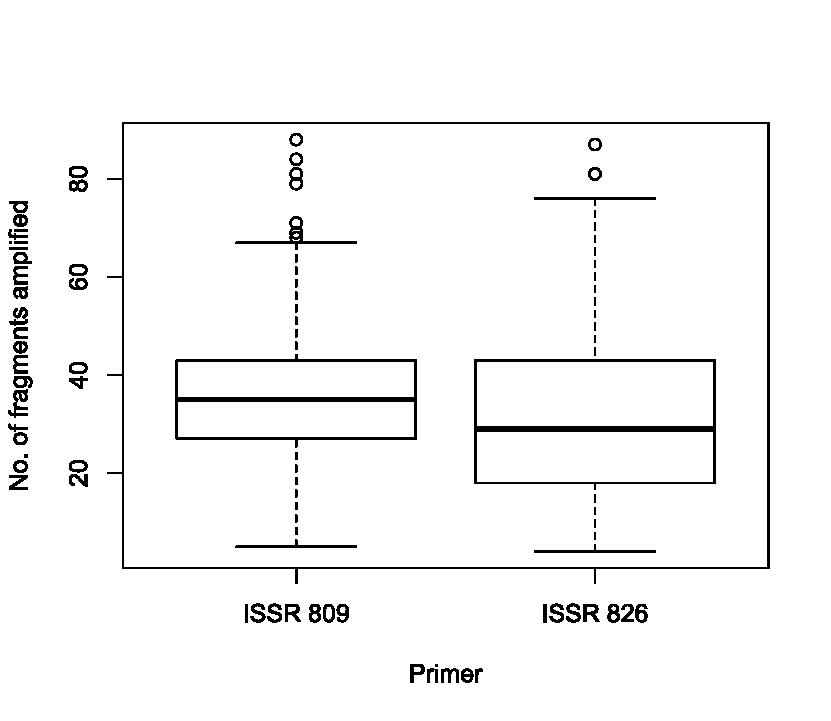
\includegraphics[scale =0.75]{Images/number_fragments_amplified.pdf}
	\caption{A box plot for the number of fragments amplified by the ISSR 809 and ISSR 826 primers.}
	\label{fig:primer_bands}
\end{figure}

% \begin{figure}[H]
% 	\centering
% 	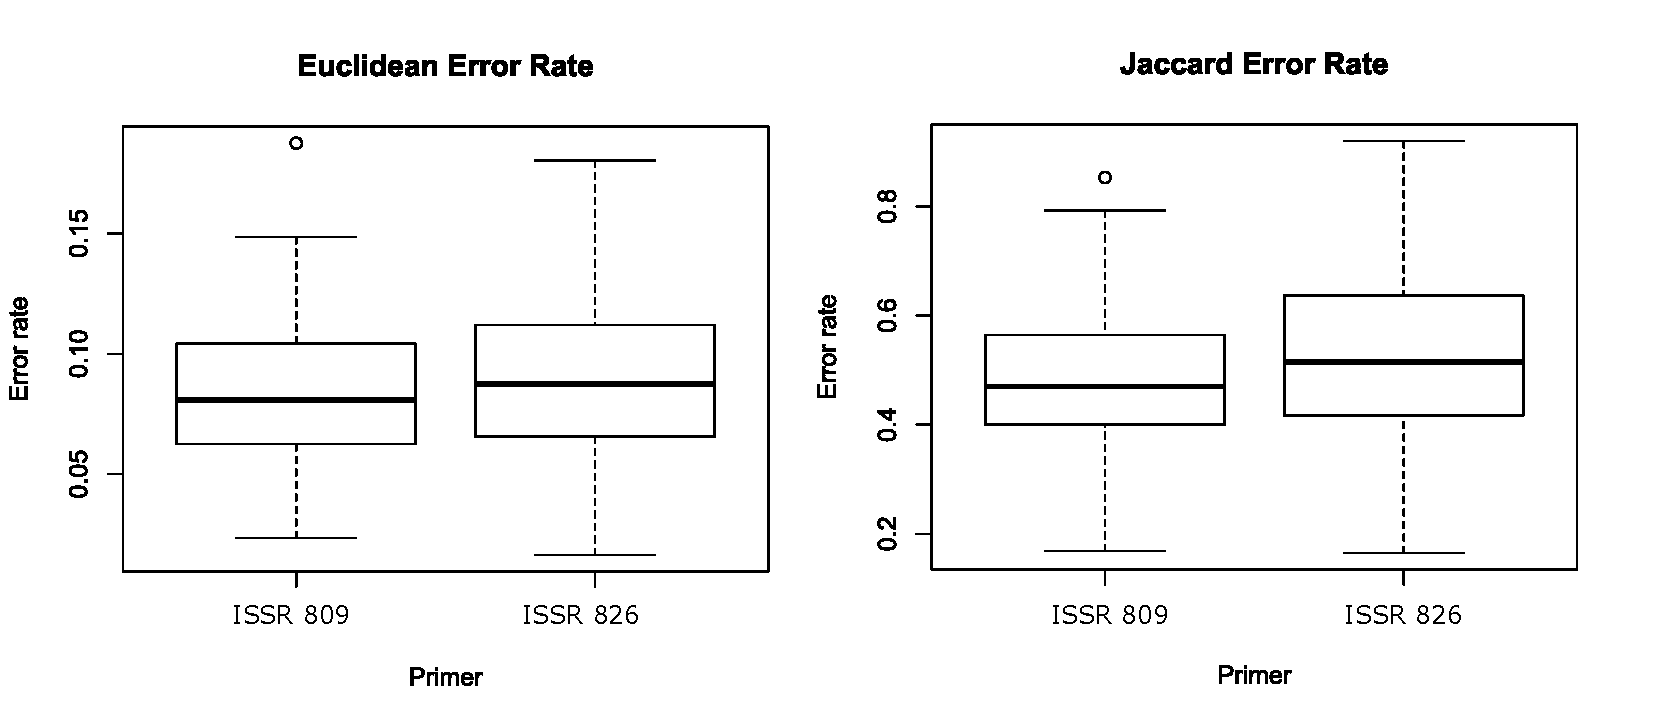
\includegraphics[scale =0.6]{Images/error_rates.pdf}
% 	\caption{Box plots for the Euclidean and Jaccard error rates for ISSR 809 and ISSR 826. Values are representative of the full data set.}
% 	\label{fig:primer_errors}
% \end{figure}

\subsection{Hierarchical clustering tree}
The UPGMA clustering tree representative of the combination of both ISSR primers showed a separation of all the \textit{Dactylopius} species (Fig. \ref{fig:issr_upgmaTree}), and corroborated the topologies in the 12S, 18S, and COI phylogenies. \textit{Dactylopius tomentosus} separated into the `californica', `imbricata', and `cholla' lineages, but `imbricata' samples split into two separate groups. The Uitenhage `ficus' and Mass Rearing Facility samples grouped together as a sister group to the Namibia `ficus' samples. The `stricta' samples from the Kruger National Park, Saudi Arabia, and samples from `stricta' source populations (kept by John Hoffmann and Hildegard Klein) separated from the `ficus' samples and from those collected in the United States. Samples from the Pecos County in Texas in the USA (VS082u and VS145) grouped with the wild `ficus' samples collected in the Eastern Cape, South Africa. Two MRF samples (Extraction IDs: VS059Os and VS063Os) grouped with samples from the USA.

\begin{figure}[H]
	\centering
	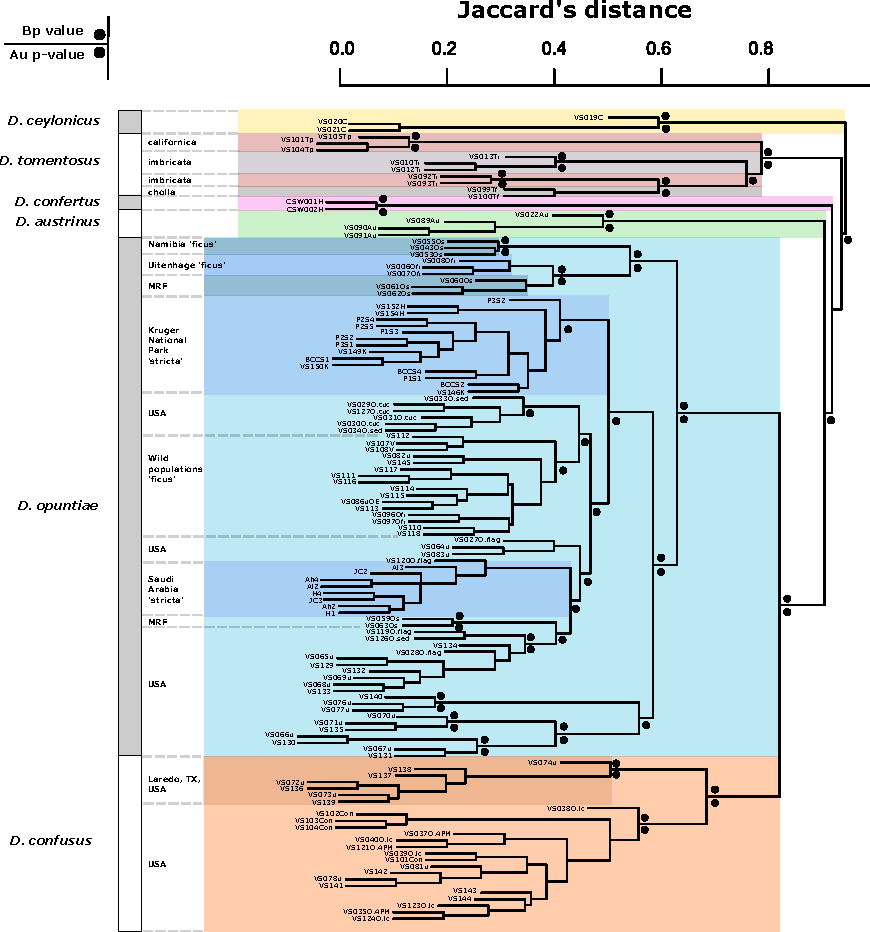
\includegraphics[height = 22cm, width = 18cm, scale =0.7]{Images/upgma_tree.pdf}
	\caption{Hierarchical clustering tree (UPGMA method) applying Jaccard's transformation for the ISSR binary data obtained from two primers (ISSR 809 and ISSR 826). Approximately unbiased p-values (Au p-value) and the bootstrap probability values (Bp-value) above 70 are shown as black dots above and below the relevant clades. One thousand bootstrap repetitions were run. MRF = Uitenhage Mass Rearing Facility.}
	\label{fig:issr_upgmaTree}
\end{figure}

\subsection{SplitsTree}
Overall, the `stricta' and `ficus' lineages showed a clear separation (Fig. \ref{fig:splitsTree}). The ANOSIM results in Table \ref{tab:ANOSIM_stats} suggest that the MRF samples were not significantly different to `ficus', but that they were to `stricta'.
The Kruger National Park and Saudi Arabian `stricta' samples separated into two groups, and the John Hoffman and Hildegard Klein samples fell into the Kruger National Park group. The wild populations, Namibian, and Uitenhage `ficus' samples also formed separate groups. See Figures \ref{fig:issr809_splitstree} and \ref{fig:issr826_splitstree} for SplitsTree diagrams for each individual ISSR primer.

\vspace{0.5cm}
\begin{figure}[H]
	\centering
	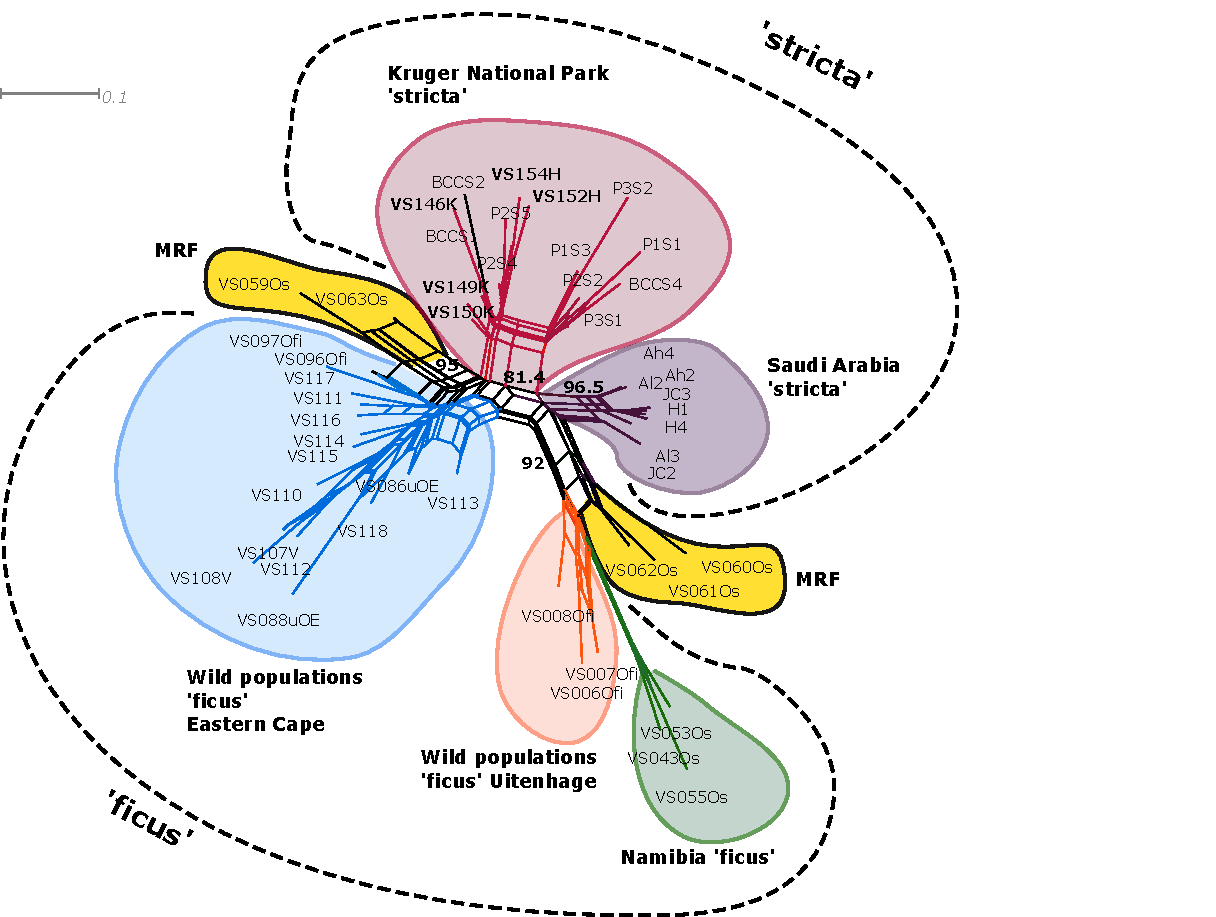
\includegraphics[scale =0.85]{Images/opuntiae_for_splitstree.pdf}
	\caption{SplitsTree graphical output (NeighborNet method, applying Jaccard's index to calculate the distance matrix) for \textit{Dactylopius opuntiae} individuals (ISSR 809 and ISSR 826). The Uitenhage and Namibia clusters are known to be the `ficus' lineage, and the Kruger National Park (KNP) contain the `stricta' lineage. Individuals in the `wild populations' group were sampled from \textit{Opuntia ficus-indica} and \textit{O. engelmannii} host plants in the Eastern Cape. MRF = the Mass Rearing Facility at Uitenhage (Eastern Cape). Bootstrap values above 75 are shown. Bold names in the KNP group denote the known `stricta' source population samples (kept by Hildegard Klein and John Hoffmann).}
	\label{fig:splitsTree}
\end{figure}

\subsection{Non-metric Multi-dimensional Scaling (nMDS) Plot}
A non-metric MDS plot (Fig. \ref{fig:2D_scatter}) showed a very similar output to the SplitsTree diagram in Figure \ref{fig:splitsTree}, with the difference of one of the Uitenhage MRF samples (VS063Os) falling within the `stricta' group. 

\vspace{0.5cm}

\begin{figure}[H]
	\centering
	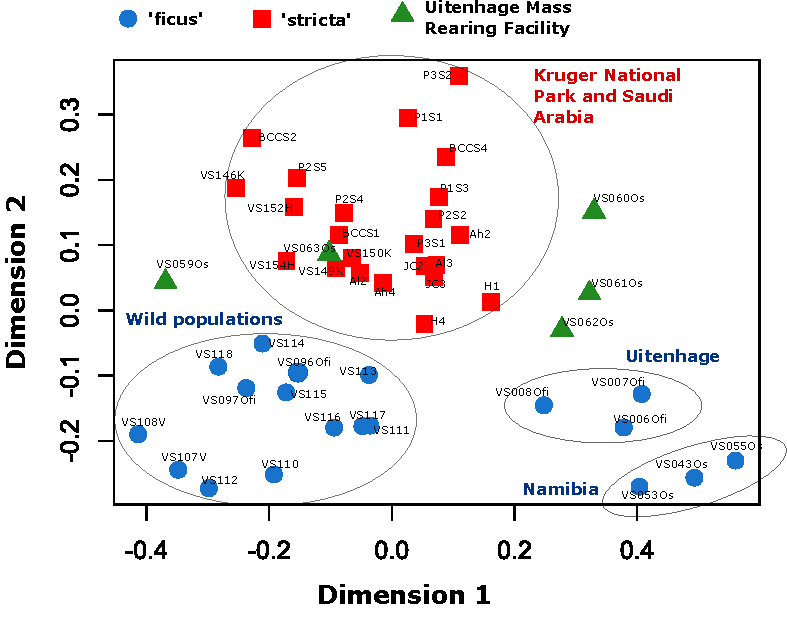
\includegraphics[scale =1.25]{Images/2d_nmds_3.pdf}
	\caption{A non-metric MDS plot based on the binary data (applying Jaccard's distance transformation) obtained from ISSR 809 and ISSR 826 to represent two different \textit{Dactylopius opuntiae} lineages. Blue circles = `ficus', red squares = `stricta', and green triangles = the Uitenhage Mass Rearing Facility.} 
	\label{fig:2D_scatter}
\end{figure}

\noindent The K = 2 dimension was applied for the nMDS plot, as the resulting stress value fell within the acceptable range (Fig. \ref{fig:shep_plots} A, B and C) \citep{dugard2010stats}. 
% Between the dimensions k = 2 and k = 3, the latter produced the lowest stress value of 0.11 compared to 0.14 (Fig. \ref{fig:shep_plots} A, B and C). The number of dimensions in a MDS analysis should ideally be kept to a minimum, and so K = 2 was applied as this stress value still falls within the acceptable range  \\
With the `ficus' group as a whole (ANOSIM: R = 0.43, p = 0.001; PERMANOVA: DF = 2, F = 6.6, R\textsuperscript{2} = 0.22, p = 0.001), and divided into known ficus samples and wild populations (ANOSIM: R = 0.72, p = 0.001; PERMANOVA: DF = 3, F = 11.69, R\textsuperscript{2} = 0.43, p = 0.001), pairwise comparisons showed that all groups were significantly different from each other (Tables \ref{tab:ANOSIM_stats}, \ref{tab:ANOSIM_stats_2}, \ref{tab:adonis_stats} and \ref{tab:adonis_stats2}). The `ficus' and MRF groups showed the greatest level of similarity (Tables \ref{tab:ANOSIM_stats} and \ref{tab:adonis_stats2}).

\begin{table}[H]
\renewcommand{\arraystretch}{0.5}
\centering
\caption{ANOSIM intra-group statistics for \textit{D. opuntiae} `stricta', `ficus' and Mass Rearing Facility (MRF) groups, showing their R values, followed by uncorrected p-values in brackets. Permutations = 999. Overall R value = 0.44, p = 0.001. Asterisks denote significance (p $<$ 0.05).}
\label{tab:ANOSIM_stats}
\begin{tabular}{@{}llll@{}}
\toprule
 & \textbf{`stricta' \scriptsize{(n = 23)}} & \textbf{`ficus' \scriptsize{(n = 21)}} & \textbf{MRF \scriptsize{(n = 5)}} \\ \midrule
\textbf{`stricta'} &  &  &  \\
\textbf{ficus} & 0.46 (0.0001)* &  & \\
\textbf{MRF} & 0.57 (0.0001)* & 0.20 (0.066) & \\ \bottomrule
\end{tabular}
\end{table}

\begin{table}[H]
\renewcommand{\arraystretch}{0.5}
\centering
\caption{ANOSIM intra-group statistics for \textit{D. opuntiae}, where the `ficus' group is split into wild populations and the `ficus' collected from around Uitenhage and in Namibia. R values are shown, followed by uncorrected p-values in brackets. Permutations = 999. Overall R value = 0.72, p = 0.001. Asterisks denote significance (p $<$ 0.05).}
\label{tab:ANOSIM_stats_2}
\begin{tabular}{@{}lllll@{}}
\toprule
 & \textbf{`stricta' \scriptsize{(n = 23)}} & \textbf{`ficus' \scriptsize{(n = 6)}} & \textbf{MRF \scriptsize{(n = 5)}} & \textbf{Wild \scriptsize{(n = 15)}} \\ \midrule
\textbf{`stricta'} &  &  &  &  \\
\textbf{`ficus'} & 0.90 (0.0001)* &  &  & \\
\textbf{MRF} & 0.57 (0.0001)* & 0.43 (0.0043)* &  &  \\
\textbf{Wild} & 0.66 (0.0001)* & 0.96 (0.0001)* & 0.74 (0.0002)* &  \\ \bottomrule
\end{tabular}
\end{table}

\begin{table}[H]
\renewcommand{\arraystretch}{0.5}
\centering
\caption{Permutational Multivariate Analysis Of Variance Using Distance Matrices for \textit{D. opuntiae} `stricta', `ficus' and Mass Rearing Facility (MRF) groups. Pairwise p-values are shown. Permutations = 999, DF = 2, F = 6.60, R\textsuperscript{2} = 0.22, p = 0.001. Asterisks denote significance (p $<$ 0.05).}
\label{tab:adonis_stats}
\begin{tabular}{@{}lll@{}}
\toprule
 & \textbf{`stricta'} & \textbf{`ficus'} \\ \midrule
\textbf{`ficus'} & 0.003* &   \\
\textbf{MRF} & 0.003* & 0.045*   \\ \bottomrule
\end{tabular}
\end{table}

\begin{table}[H]
\renewcommand{\arraystretch}{0.5}
\centering
\caption{Permutational Multivariate Analysis Of Variance Using Distance Matrices intra-group statistics for \textit{D. opuntiae} where the `ficus' group is split into wild populations and the `ficus' collected from around Uitenhage and in Namibia. MRF = Mass Rearing Facility. Pairwise p-values are shown. Permutations = 999, DF = 3, F = 11.69, R\textsuperscript{2} = 0.43, p = 0.001. Asterisks denote significance (p $<$ 0.05).}
\label{tab:adonis_stats2}
\begin{tabular}{@{}llll@{}}
\toprule
 & \textbf{`stricta'} & \textbf{ficus} & \textbf{MRF} \\ \midrule
\textbf{`ficus'} & 0.0012* & &  \\
\textbf{MRF} & 0.0012* & 0.006* &  \\
\textbf{Wild} & 0.0012* & 0.0012* & 0.0012* \\ \bottomrule
\end{tabular}
\end{table}

% With all `ficus' samples grouped (all the samples collected from \textit{O. ficus-indica} and \textit{O. engelmannii}), a one-way ANOSIM (9999 permutations applying the Jaccard similarity index) showed that the MRF samples were more similar to the `ficus' group (R = 0.20, p = 0.066) than they were to the `stricta' group (R = 0.57, p = 0.0001) (Table \ref{tab:ANOSIM_stats}). When the `ficus' group was divided into two, namely 1) the wild populations and 2) known `ficus' samples from Uitenhage and Namibia, the MRF samples were significantly different (R = 0.76, p = 0.0002) from the wild populations, and showed more similarity to the `ficus' samples from \textit{O. ficus-indica} in Uitenhage and Namibia (R = 0.43, p = 0.0043) than to `stricta' (R = 0.57, p = 0.0001). (Table \ref{tab:ANOSIM_stats_2}). `Stricta' and `ficus' showed significant dissimilarity to each other (R = 0.90, p = 0.0001). Corroborating with the Bayesian structure results (Fig. \ref{fig:struc}), the wild populations were more similar to `stricta' (R = 0.66, p = 0.0001) than to `ficus' (R = 0.96, p = 0.0001).

% \begin{figure}[H]
% 	\centering
% 	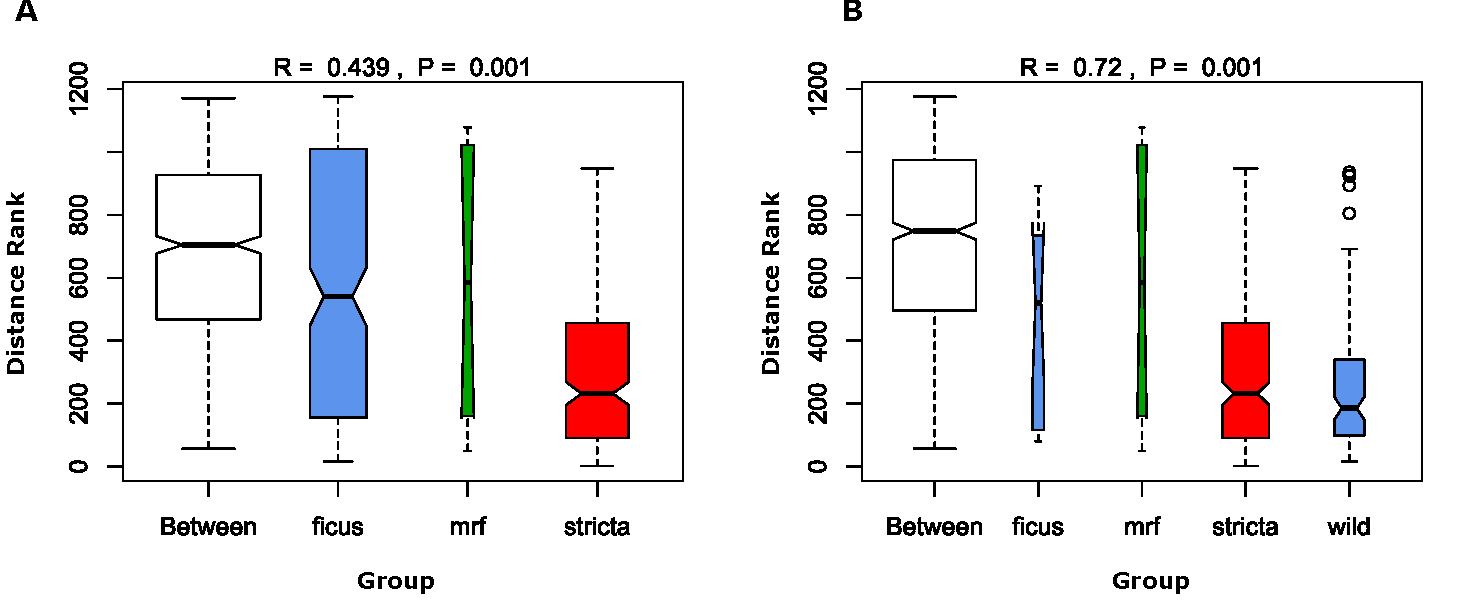
\includegraphics[scale =0.65]{Images/Anosim_opuntiae_1.pdf}
% 	\caption{Analysis of Similarity (ANOSIM) boxplots for the distances between and within A) `stricta', `ficus' and Mass Rearing Facility (MRF) groups, and B) where the `ficus' cluster is divided into samples from Uitenhage and Namibia (`ficus') and from wild populations collected in the Eastern Cape (`wild'). Black horizontal bars in the boxes indicate the median, and the bottom and top of each box represents the 25th and 75th percentile. The whiskers extend to the most extreme data points, with outliers shown as open circles. The widths of the bars are directly proportional to sample size.}
% 	\label{fig:ranked_distances}
% \end{figure}

\subsection{Structure plots}
With population data not set as priors, the \citet{puechmaille2016program} method indicated an optimal \textit{K}-value of 5, set at a threshold of 0.6, for all four tests (the MedMedK, MedMeanK, MaxMedK and MaxMeanK). The \citet{evanno2005detecting} method indicated optimal \textit{K}-values of 2 and 6 according to the $\Delta$\textit{K} and mean LnP(\textit{K}) methods, respectively. \\
When population data were set as priors, the \citet{puechmaille2016program} method gave the same output as above, except that the \citet{evanno2005detecting} method gave the optimal \textit{K}-value as being 2 for the $\Delta$\textit{K} method, and 5 for the mean LnP(\textit{K}) method. Clusters \textit{K} = 2 and \textit{K} = 5 are presented in the resulting Structure plots (Fig. \ref{fig:struc}). 
In both Structure plots (with and without priors), when \textit{K} = 2, the Saudi Arabia, Kruger National Park and Klein and Hoffmann source populations of `stricta' formed one shared cluster (light blue). The Uitenhage and Namibia `ficus' and three of the MRF samples formed a second cluster (orange). Two of the MRF samples shared the same cluster group as `stricta'. When forced into one of two clusters, the wild `ficus' populations were more genetically similar to the `stricta' cluster than they were to `ficus' samples. \\
When \textit{K} = 5, the Kruger National Park and Klein and Hoffmann source population `stricta' samples formed one cluster (maroon) (Fig. \ref{fig:struc}). The Uitenhage `ficus' and three of the MRF samples formed a separate cluster (orange). The remaining two MRF samples shared a cluster with the wild `ficus' populations (light blue). The MRF samples shared some similarity to the Kruger National Park and Saudi Arabian `stricta' clusters. The Saudi Arabian `stricta' (dark purple) and Namibian `ficus' (green) formed their own separate clusters. Taking into account Figures \ref{fig:splitsTree} and \ref{fig:struc}, individuals from the Uitenhage MRF appear to be either a hybrid of the `stricta' and `ficus' lineages, or they fall within the `ficus' group. 

\subsection{Identification accuracy}
At the species level, at an optimal threshold of 60\%, all barcode tests (BCM, TID, and NN) had a 100\% IA (Table \ref{tab:issr_barcode_results}). At the lineage level, at an optimal threshold of 45\%, \textit{D. tomentosus} had an IA of 100\% for both the BCM and TID tests (Table \ref{tab:issr_barcode_results}). At the same 45\% threshold, \textit{D. opuntiae} had an IA of 81.82\% (no ID of 18.18\%) for both the BCM and TID tests.

\vspace{0.5cm}
\begin{table}[H]
\renewcommand{\arraystretch}{0.5}
\caption{Barcode testing results for the Best Close Match (BCM), Threshold ID (TID), and Nearest Neighbour (NN) tests, at the species and lineage level.}
\label{tab:issr_barcode_results}
\resizebox{\columnwidth}{!}{%
\begin{tabular}{lllllllll}
\hline
 &  & \textbf{BCM} & \textbf{\% of samples} & \textbf{TID} & \textbf{\% of samples} & \textbf{} & \textbf{NN} & \textbf{\% of samples} \\ \hline
\textbf{SPECIES LEVEL} & \textbf{} & \textbf{60\% threshold} &  & \textbf{60\% threshold} &  &  &  &  \\
 & \textbf{Correct} & 124 & 100 & 124 & 100 & \textbf{True} & 124 & 100 \\
\textbf{} & \textbf{No id} & 0 & 0 & 0 & 0 & \textbf{False} & 0 & 0 \\
 & \textbf{} &  &  &  &  & \textbf{} &  &  \\
\textbf{LINEAGE LEVEL} & \textit{\textbf{D. tomentosus}} & \textbf{45\% threshold} &  & \textbf{45\% threshold} &  & \textbf{} &  &  \\
 & \textbf{Correct} & 10 & 100 & 10 & 100 & \textbf{True} & 10 & 100 \\
 & \textbf{Incorrect} & 0 & 0 & 0 & 0 & \textbf{False} & 0 & 0 \\
\textbf{} & \textbf{Ambiguous} & 0 & 0 & 0 & 0 &  &  &  \\
 & \textit{\textbf{}} &  &  &  &  &  & \textbf{} &  \\
 & \textit{\textbf{D. opuntiae}} & \textbf{45\% threshold} &  & \textbf{45\% threshold} &  &  &  &  \\
 & \textbf{Correct} & 36 & 81.82 & 36 & 81.82 & \textbf{True} & 44 & 100 \\
 & \textbf{Incorrect} & 0 & 0 & 0 & 0 & \textbf{False} & 0 & 0 \\
 & \textbf{Ambiguous} & 0 & 0 & 0 & 0 &  &  &  \\
 & \textbf{No id} & 8 & 18.18 & 8 & 18.18 &  & \textbf{} & \\ \bottomrule
\end{tabular}
}
\end{table}

\vspace{0.5cm}
\begin{figure}[H]
	\centering
	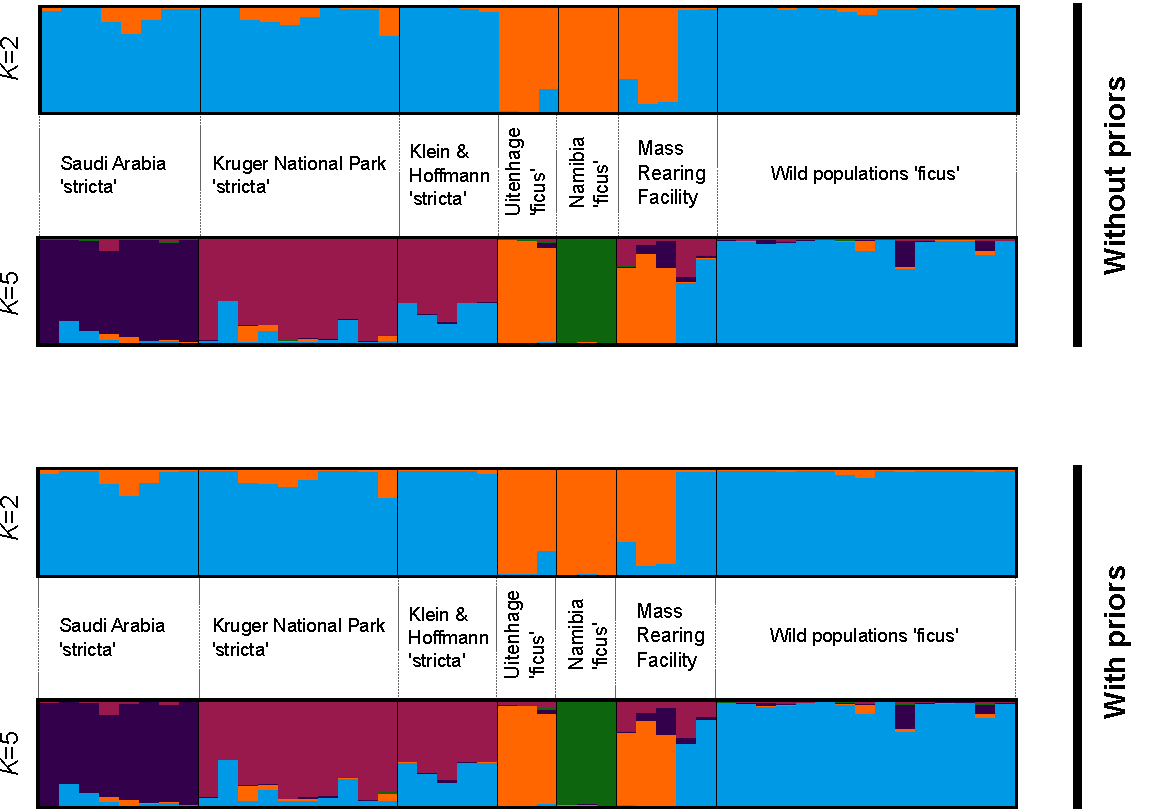
\includegraphics[scale =0.9]{Images/structure_diagrams.pdf}
	\vspace{0.2cm}
	\caption{STRUCTURE results using Bayesian analysis (MCMC = 50 000, burn-in = 100 000), showing genetic clustering patterns for \textit{Dactylopius opuntiae} individuals. Results for both \textit{K} = 2 and \textit{K} = 5 are shown for runs with and without priors.}
	\label{fig:struc}
\end{figure}


%\end{landscape}

